\documentclass[paper=a4, fontsize=11pt]{scrartcl}
\usepackage[T1]{fontenc}
\usepackage{fourier}
\usepackage[english]{babel}	
% English language/hyphenation
\usepackage[protrusion=true,expansion=true]{microtype}	
\usepackage{amsmath,amsfonts,amsthm} % Math packages
\usepackage[pdftex]{graphicx}	
\usepackage{url}

\usepackage[section]{placeins}

\usepackage[bottom=1.5in, top=1.5in]{geometry}

\usepackage{enumitem}

\newlength\tindent
\setlength{\tindent}{\parindent}
\setlength{\parindent}{0pt}
\renewcommand{\indent}{\hspace*{\tindent}}

%%% Custom sectioning
\usepackage{sectsty}
%\allsectionsfont{\centering \normalfont\scshape}


%%% Maketitle metadata
\newcommand{\horrule}[1]{\rule{\linewidth}{#1}} 	% Horizontal rule

\title{
		%\vspace{-1in} 	
		\usefont{OT1}{bch}{b}{n}
		\normalfont \normalsize \textsc{The University of Texas at Austin} \\ [25pt]
		\horrule{0.5pt} \\[0.4cm]
		\huge Statistical Modeling II Project \\
		\horrule{2pt} \\[0.5cm]
}
\author{
		\normalfont 								\normalsize
        Juliette Franqueville\\[-3pt]		\normalsize
        \today
}
\date{}


%%% Begin document
\begin{document}
\maketitle
\newpage
\section{Introduction}

The COVID-19 pandemic resulted in stay-at-home orders across the world. As a result, people spent more time at home and in outdoor areas and less time commuting to work or restaurants. This report explores the relationship between the changes in mobility patterns of the general population and the number of incidents reported by fire departments in the United States in 2020. Several studies have already explored the effect of COVID-19 on fire incidents. For example, Suzuki and Manzello \cite{fire_paper} analyzed the effect of stay-at-home orders on cooking fires in major cities. Koester and Greatbatch \cite{koester2020comparing} investigated the impact of the onset of the pandemic on fire and search and rescue incident frequency. This report utilizes NFORS \cite{nfors} analytics data provided by the International Public Safety Data Institute and 2020 Google Mobility data \cite{google}. The names of the fire departments were hidden for anonymity. 

\section{Data Formatting}
The raw datasets were formatted to obtain weekly averages for number of incident percentage change from baseline for 2020 for each fire department in NFORS and 2020 weekly average Google mobility data corresponding to the county of each NFORS department.\\


The Google data columns of interest were date,  FIPS code (which corresponds to unique county) and percentage change from baseline for workplace, residential, retail, parks, and grocery/pharmacy mobility. First, the Google mobility data were grouped by FIPS codes.  The data with FIPS codes corresponding to those of the counties of the fire departments in the NFORS data were kept.\\



The Google mobility data is reported as a percentage change from baseline. The baseline used is the median value for each day of the weeks over the January 3rd - February 6th 2020 period. To get a weekly average, a 7-day rolling average was used and the value for all Mondays was reported as the weekly average. \\

In the NFORS data, the data of interest were date, fire department, and number of incidents reported for each date. Note that all types of incidents (fire, car crashes, and EMS) were pooled together in the incident counts. For each fire department, gaps in data (where more than two consecutive days had zero incidents, which is very unlikely) were removed. Then, outliers were removed by fitting a negative binomial distribution to the incident counts of each department using moment matching and removing points outside the 95 \% confidence interval.\\


An incident baseline was calculated from the 2019 NFORS data and applied to the 2020 data. The baseline was calculated by taking the median of the number of incidents per day of the week per month for each department. Accounting for month as well as day of the week ensured that the seasonality in fire incidents was accounted for. Then, the percentage change for each day in 2020 was calculated from this baseline. Note that some departments were missing significant amounts of data and did not allow for calculating a baseline for each month and each day of the week in 2019. For missing baseline data points, the corresponding changes from baseline in 2020 could not be calculated.  Some department had no data for 2019, so they were not used in the analysis, As with the Google data, a weekly average for incident percentage change form baseline for each department was calculated. \\

 The resulting data format was an $X_i \in \mathbb{R}^{n_i \times p}$ matrix for each department, where $p$ is the number of mobility types (workplace, retails, etc), $i$ is the department, and $n_i$ is the number of weekly averages for each department. Note that ideally, each department would have $n_i = 52$ because there are 52 weeks in a year, but the Google mobility data only begins in February 2020 and some departments had missing data. Each department also had a $y_i \in \mathbb{R}^{n_i}$ vector of incident percentage change from baseline corresponding to the $X_i$ matrices. Additionally, each department had a $t_i \in \mathbb{R}^{n_i}$ vector containing the day of the year that the observations are for (days all correspond to Mondays because the weekly averages were evaluated on Mondays).


\section{Data Exploration}
The various mobility types were highly correlated. Figure \ref{corr_mat} shows the correlation matrix for the mobility types for all departments. The correlations are as expected; for example workplace mobility is inversely correlated with residential mobility. Parks, however, is not highly correlated with the other mobility types.


\begin{figure}[!htb]\label{corr_mat}
\centering
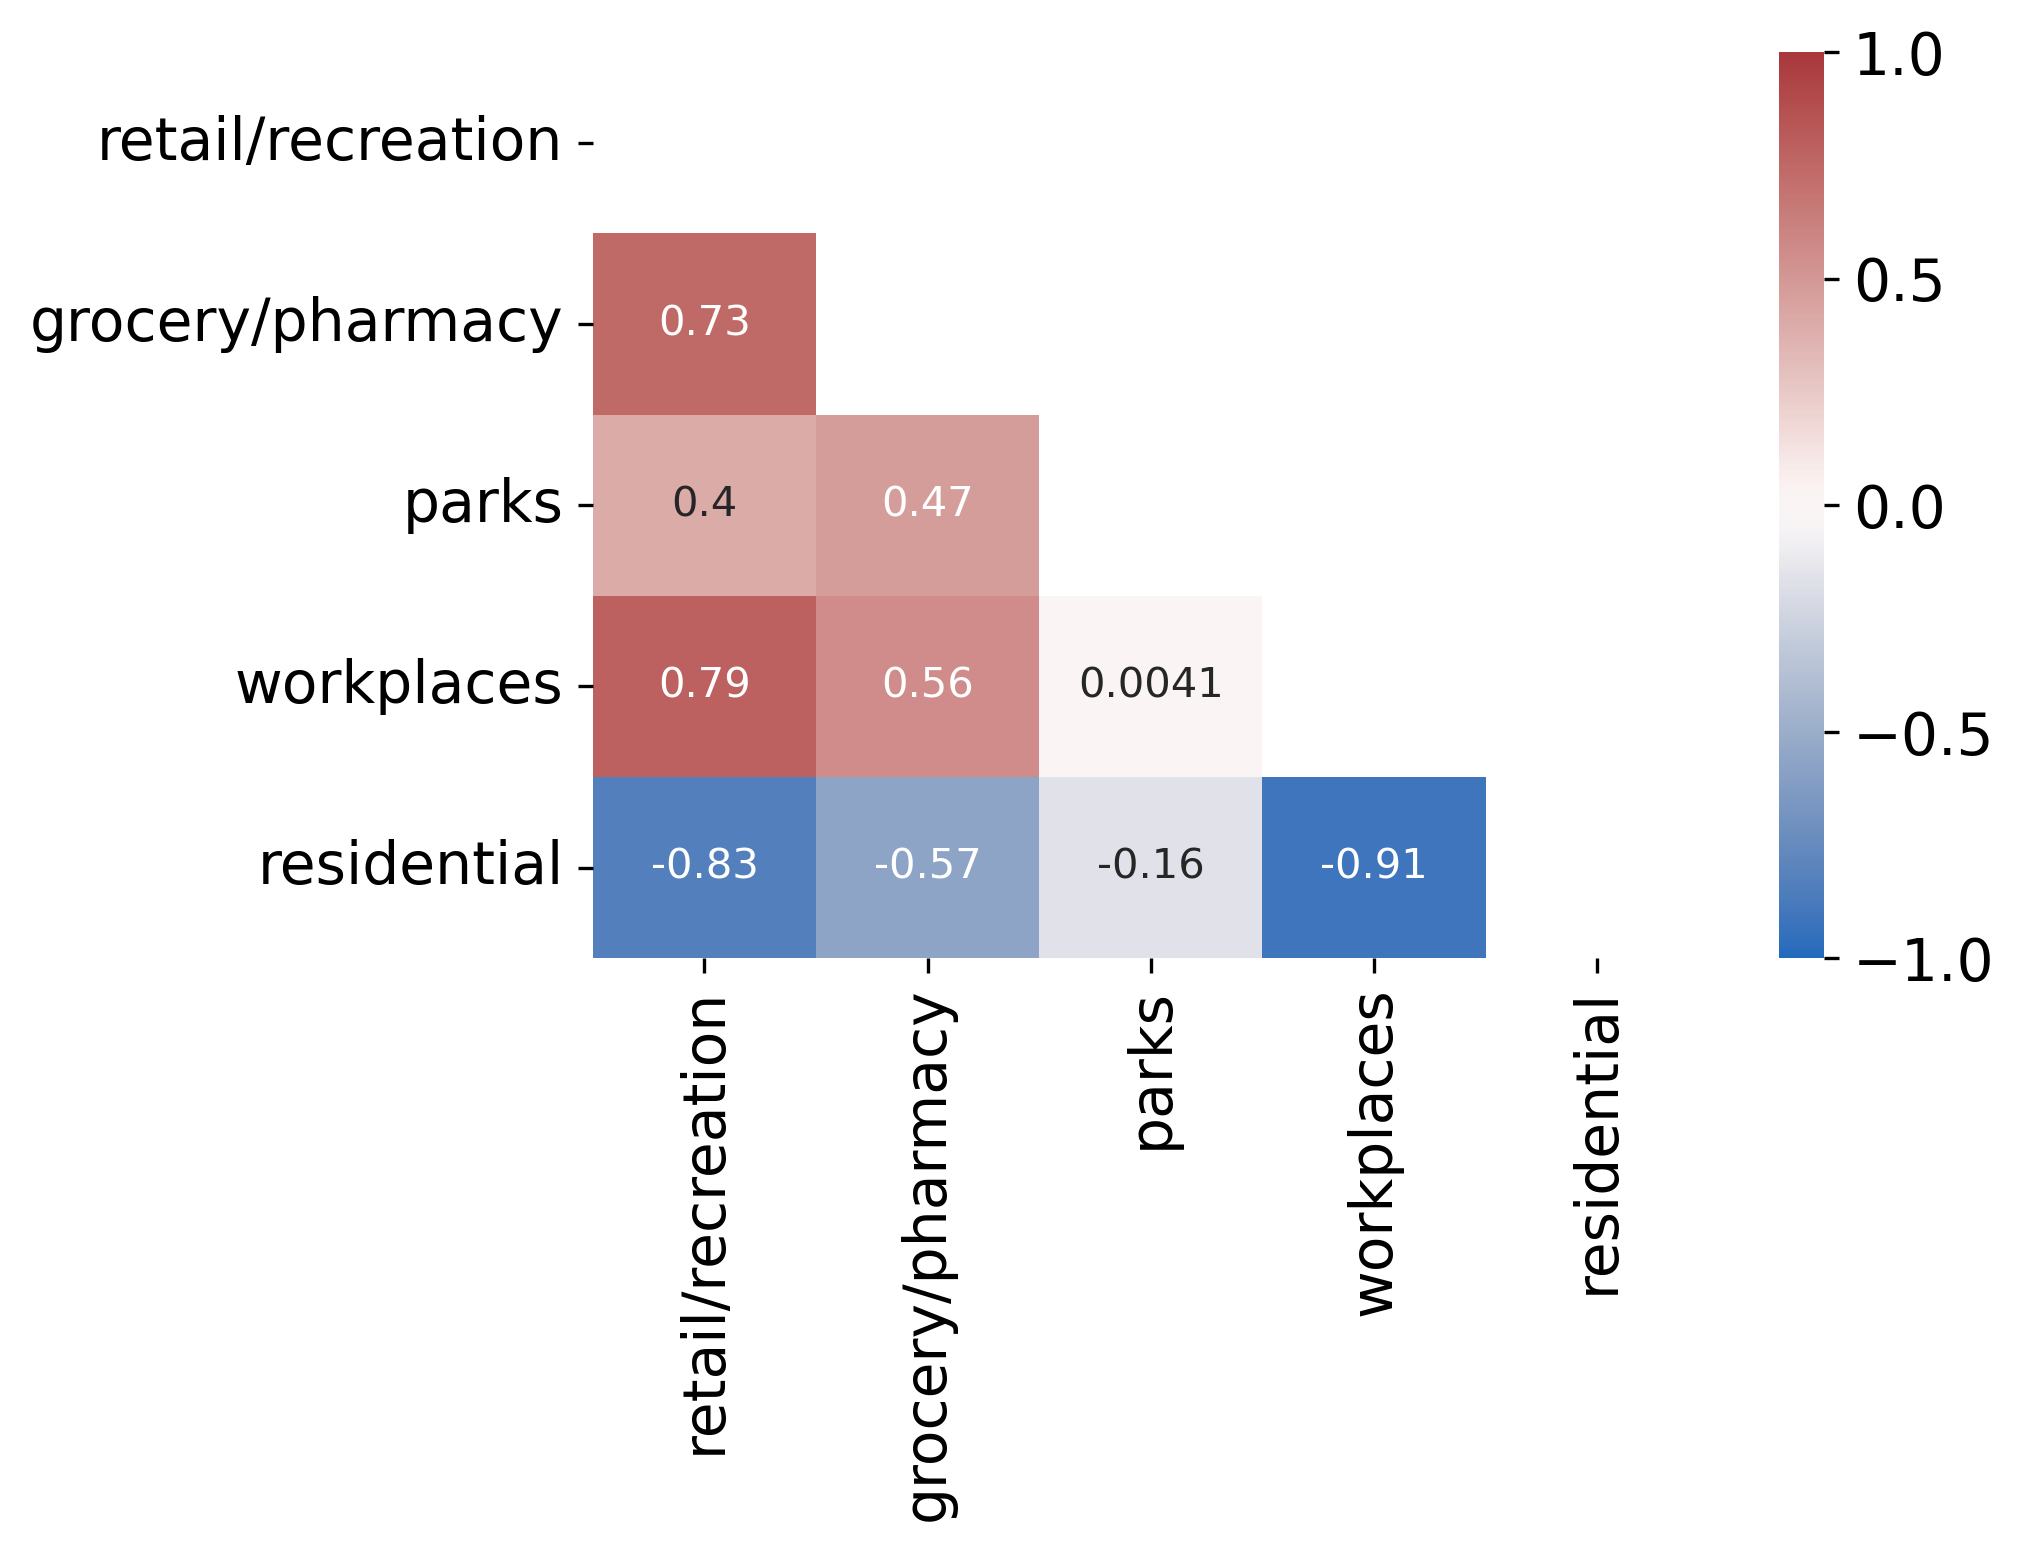
\includegraphics[width=.7\textwidth]{corr.png}
\caption{Correlation Matrix}
\end{figure}

To avoid multicolinearity issues in the model, principal component analysis was performed and the first two components were kept. The components were calculated by first subtracting the mean of each mobility type from the corresponding mobility values. Then, the covariance matrix for the centered data was calculated. Then, the eigenvalues (or the explained variance corresponding to each component) and the eigenvectors (components) of the covariance matrix were calculated. The two components corresponding to the two highest eigenvalues were kept. The first two components explained 99\% of the variance. The first component  pointed in the direction of ``parks'' and the second pointed in the direction of ``retail/recreation'', ``grocery/pharmacy'', ``workplaces'' and away from ``residential''. The first component can easily be interpreted as park mobility, and the second as increasing ``city'' mobility and decreasing residential mobility. The original data were transformed using the chosen components.\\

The next step was to determine whether the incident data could be approximated as being normally distribution, where:
\begin{align*}
    y_i \sim N(X_i \beta_i, \sigma_i^2I)
\end{align*}
Where $i$ is the fire department, $X_i$ is the design matrix including an intercept and transformed mobility data, $y_i$ is the response vector, $\beta_i \in \mathbb{R}^{p}$, and $I$ is the $n_i \times n_i$ identity matrix.  OLS was used separately on each department's data. As shown in Figure \ref{normal}, the Q-Q plots showed  that the residuals were approximately normally distributed; therefore no further transformations of the data were necessary.\\

Another concern was that the residuals (as plotted in Figure \ref{normal} - although some departments showed worse correlation than the 9 plotted) may be auto-correlated, in which case assuming that the covariance matrix is diagonal was not appropriate. Figure \ref{autocorr} shows ACF plots for all departments. Some departments (for example, departments 12, 13, 25, 29) had multiple correlation coefficients outside the 95 \% confidence internal. For some departments, auto-correlation was not an issue.
    
    
\begin{figure}[!htb]\label{normal}
\centering
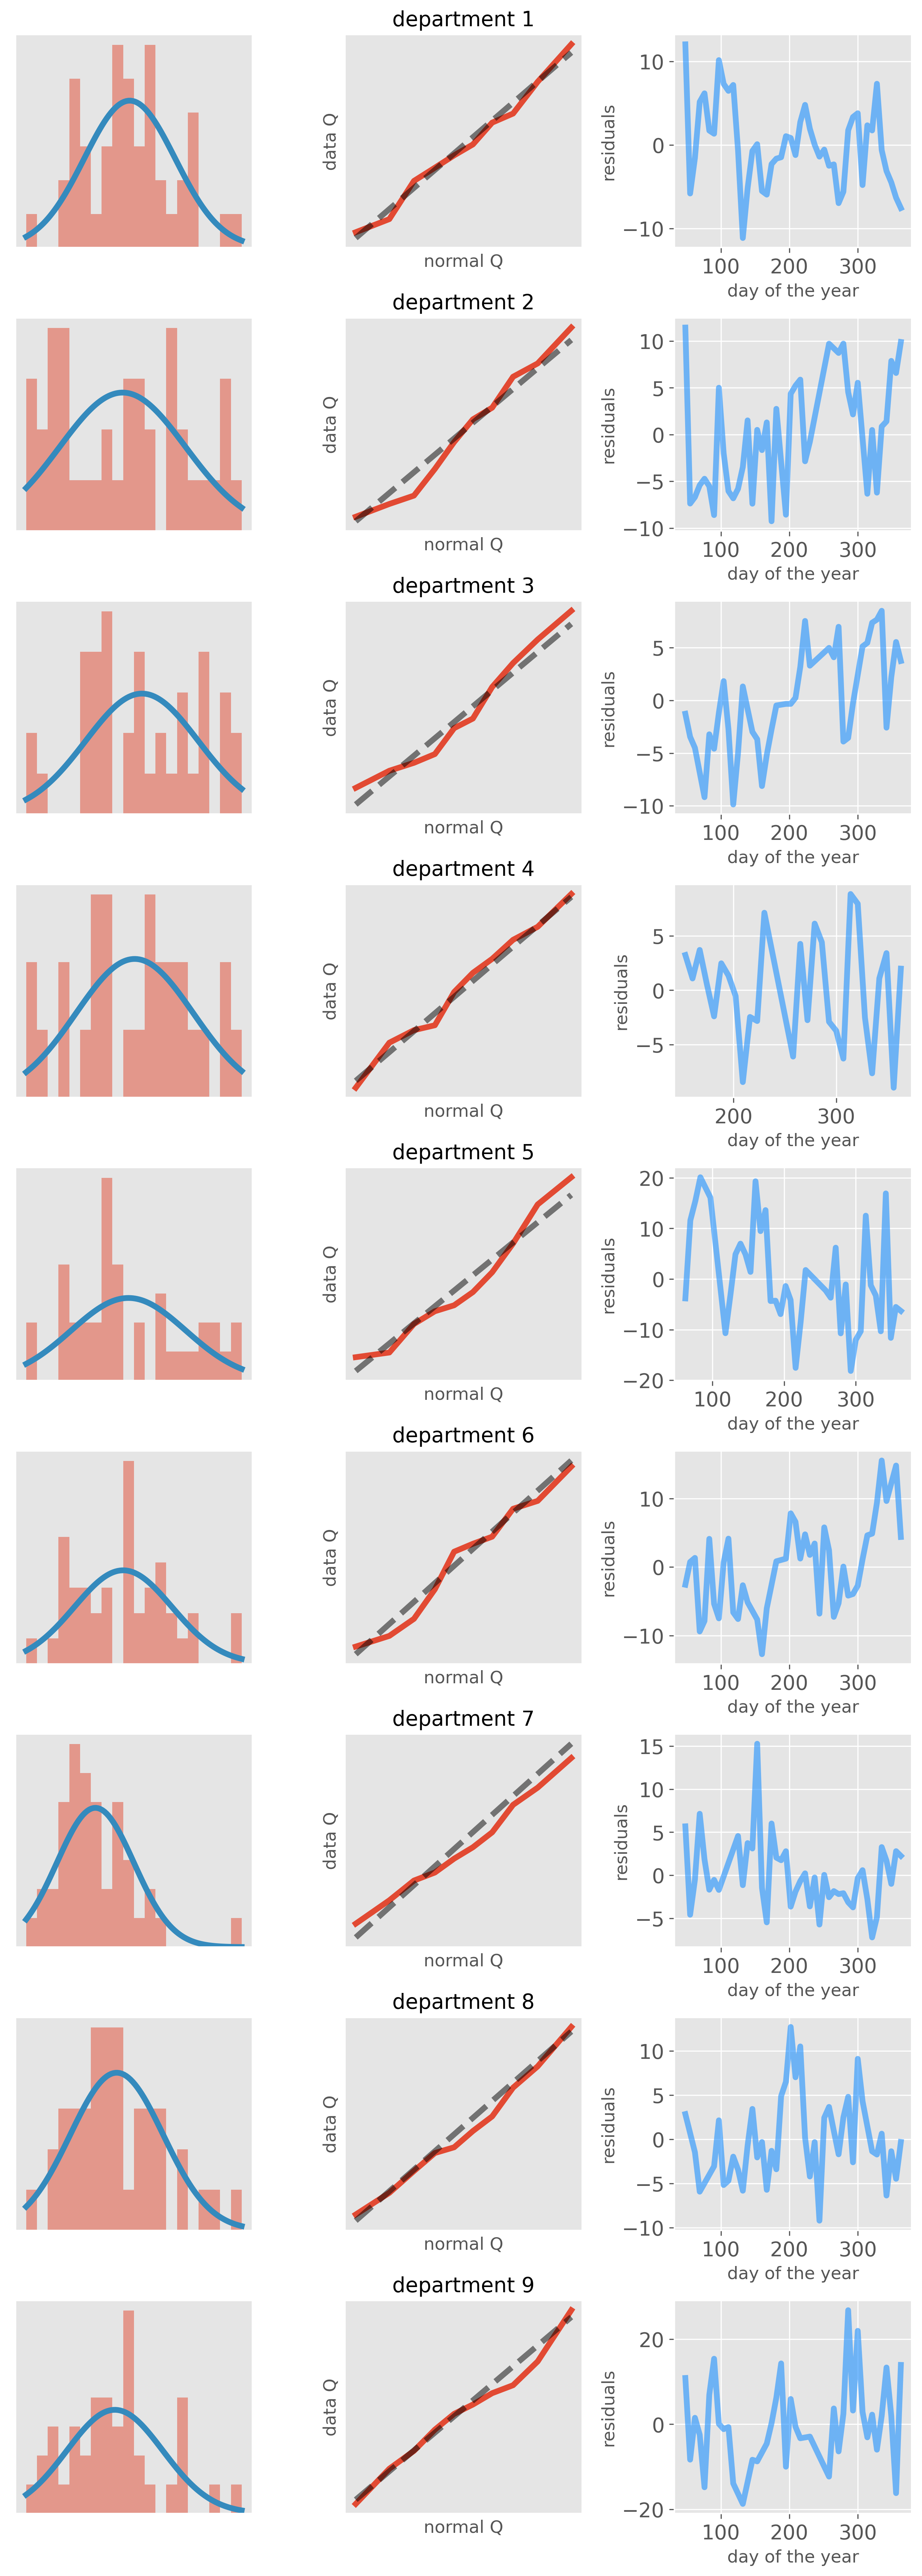
\includegraphics[width=.5\textwidth]{normal_approx_1.png}
\caption{Plots showing residuals with fitted normal with same moments as the residuals (left), Q-Q plot (middle), residuals against time (right). Only the first 9 departments are shown.}
\end{figure}


\begin{figure}[!htb]\label{autocorr}
\centering
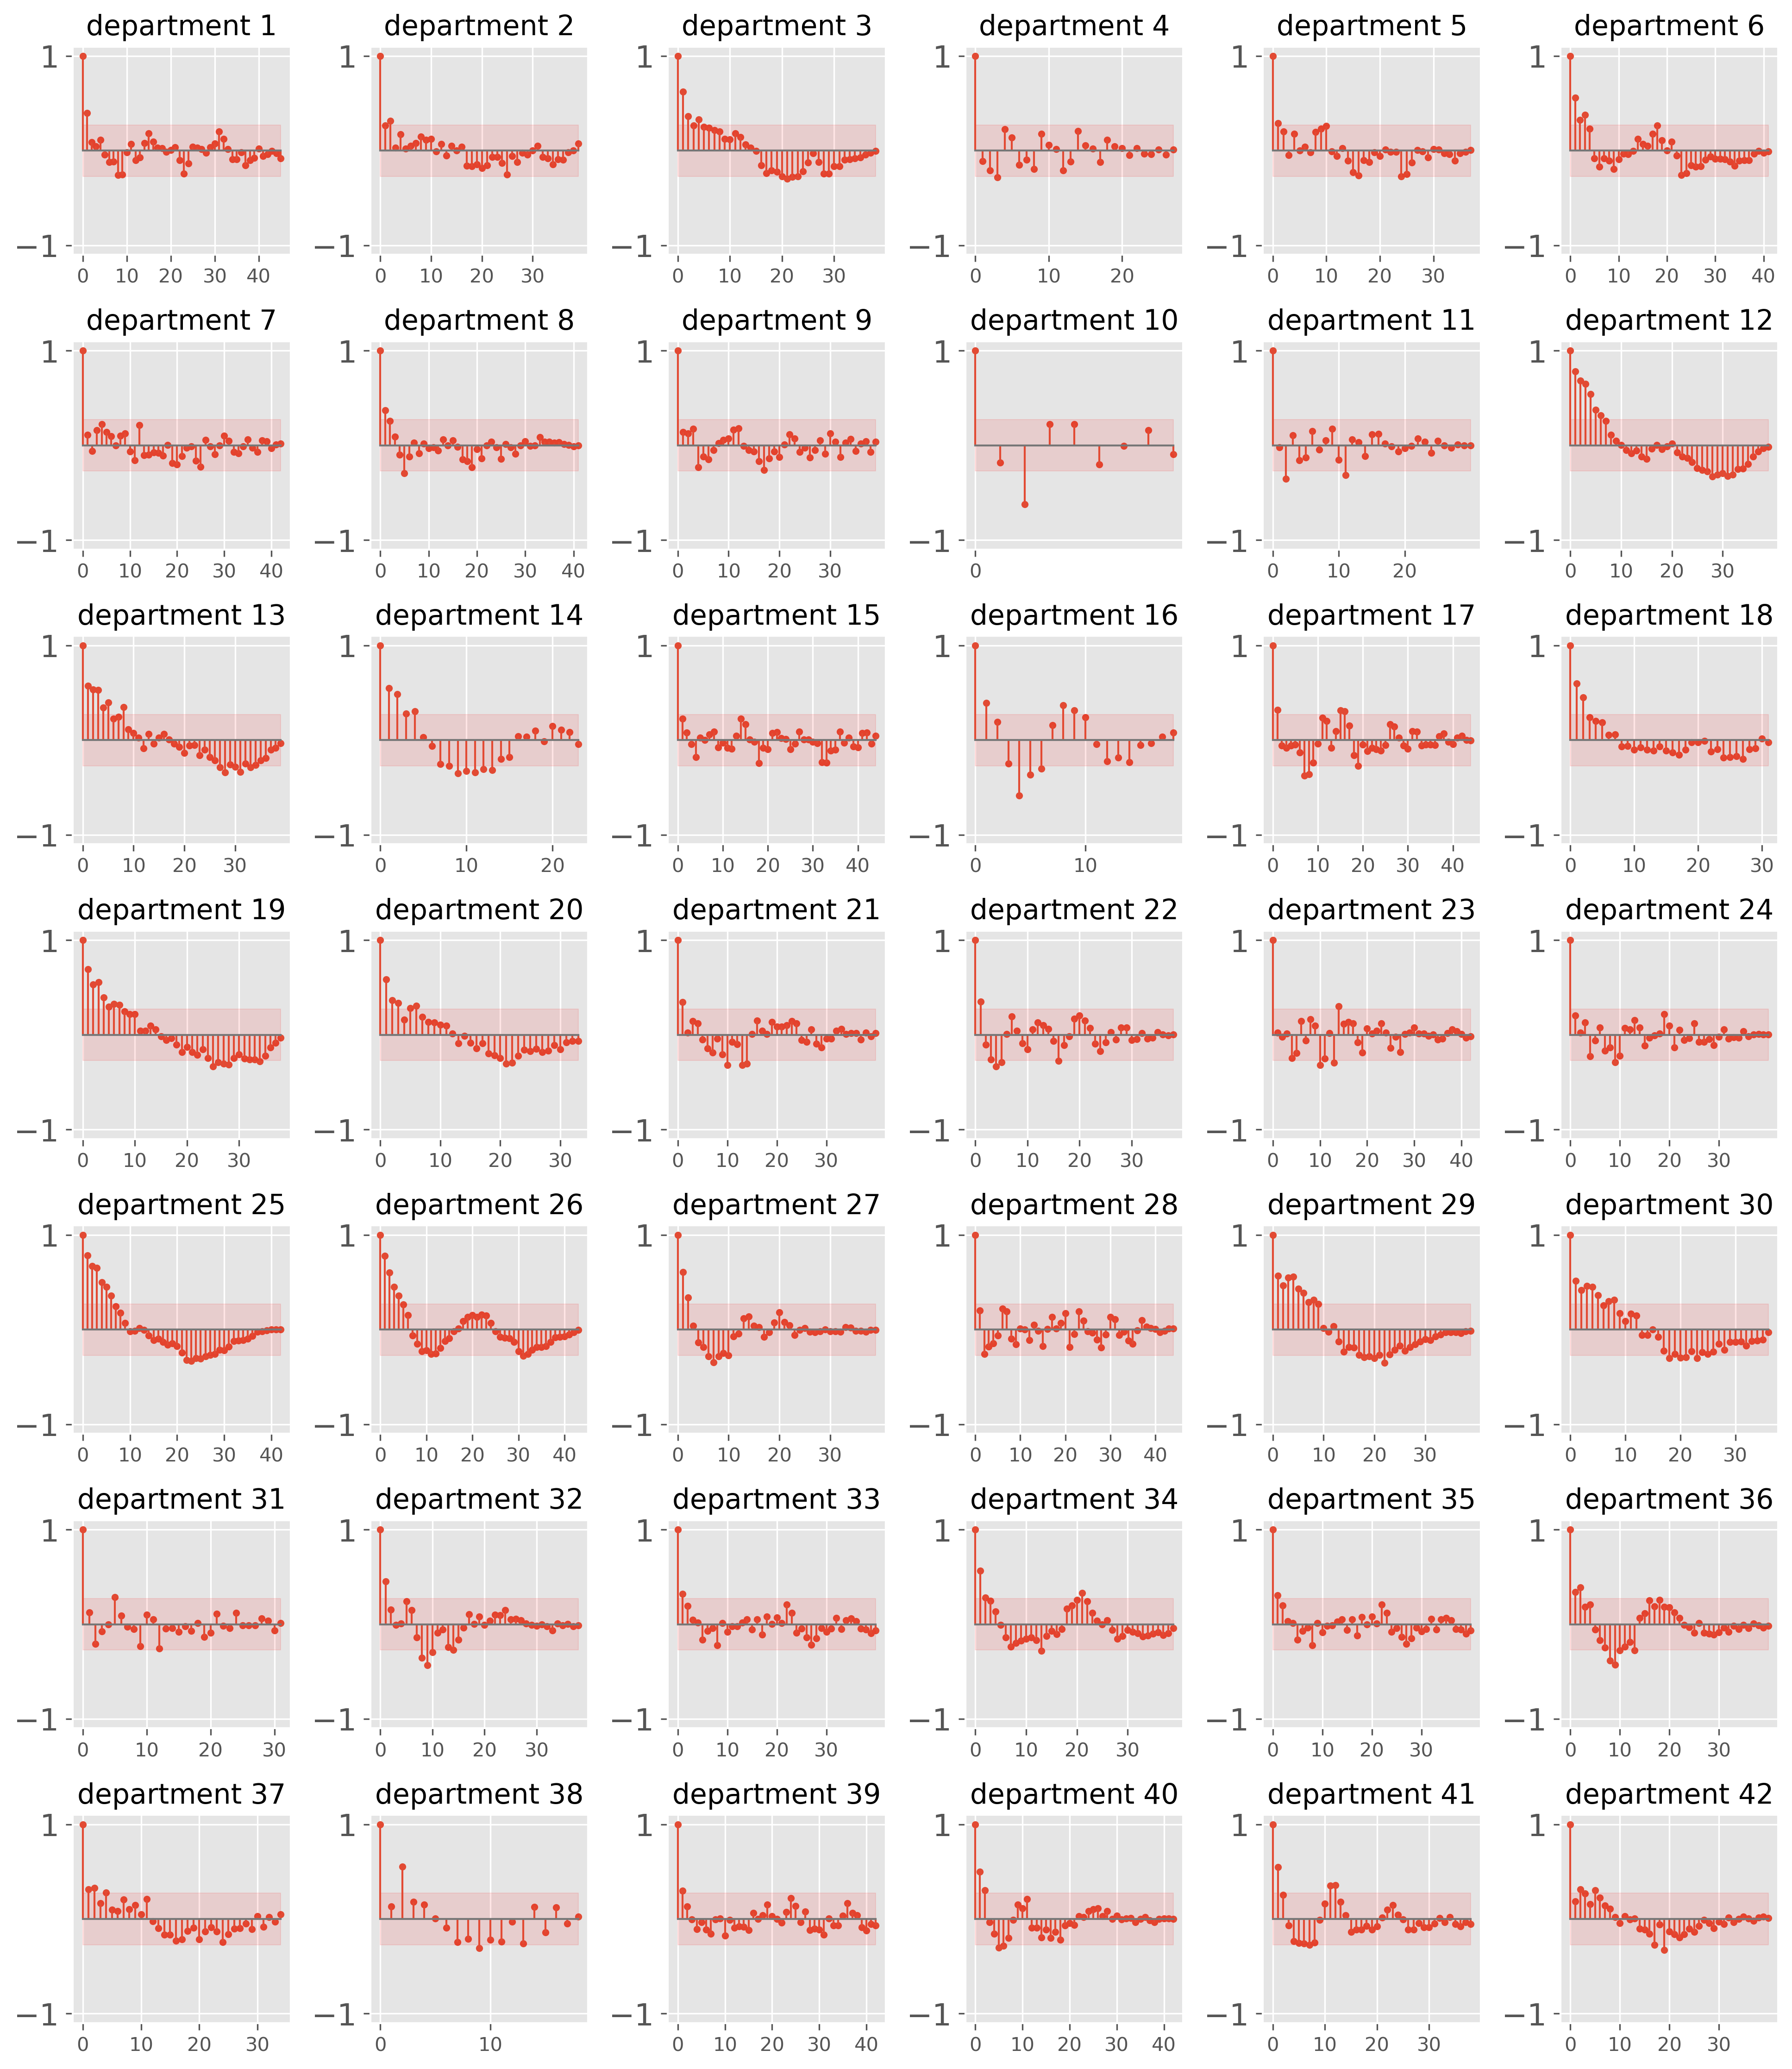
\includegraphics[width=1\textwidth]{acf_plots1.png}
\caption{ACF plots for all departments for the residuals using linear regression on each department separately.}
\end{figure}

\newpage
\section{Models}
\subsection{Simple Hierarchical Model}
As a first step before considering the autocorrelation in the residuals shown above, a simple model which did not account for auto-correlation was used:


\begin{align*}
    &y_i = X_i \beta_i+ \epsilon_i \\
     &\epsilon_i \sim N(0, \sigma^2_i I)\\
      &\beta_i \sim N(\mu, \Sigma)
\end{align*}

The following priors were used:

\begin{align*}
    & \sigma^2_i \propto \frac{1}{\sigma^2_i}\\
    & \mu \propto c \\
    & \Sigma_{jj} \sim IG \left(\frac{1}{2}, \frac{1}{2} \right)\\
\end{align*}


The conditionals needed for Gibbs sampling were

\begin{align*}
     P(\mu | \beta_i, \Sigma ) &\propto  \prod_{i=1}^{N} P(\beta_i | \mu, \Sigma)P(\mu) \\
     & \propto \prod_{i=1}^{N} \mbox{exp}\left \{-\frac{1}{2}(\beta_i - \mu)^T\Sigma^{-1}(\beta_i - \mu) \right \} \\
     & \propto \mbox{exp}\left \{-\frac{1}{2} \sum_{i=1}^{N} (\beta_i - \mu)^T\Sigma^{-1}(\beta_i - \mu) \right \}\\
     & \propto \mbox{exp}\left \{-\frac{1}{2} \sum_{i=1}^{N} \mu^T \Sigma^{-1}  \mu - 2\mu^T\Sigma^{-1} \beta_i \right \}\\
     & \propto \mbox{exp}\left \{-\frac{1}{2}\left(N \mu^T \Sigma^{-1}  \mu - 2\mu^T\Sigma^{-1} \sum_{i=1}^{N}\beta_i\right) \right \}\\
     &\sim N_p (\mu^*, \Sigma^*)
\end{align*}


Where $\mu^* = \sum_{i=1}^{N}\beta_i/N $, $\Sigma^* = \Sigma/N$ and $N$ is the number of departments.


\begin{align*}
     P(\Sigma_{jj} |\beta_{ij}, \mu_j ) & \propto  \prod_{i=1}^{N} P(\beta_{ij} | \mu_{j}, \Sigma_{jj})P(\Sigma_{jj}) \\
     & \propto \prod_{i=1}^{N} \frac{1}{\Sigma_{jj}^{1/2}} \mbox{exp} \left \{ -\frac{1}{2\Sigma_{jj} }(\beta_{ij} - \mu_j)^2 \right \} \Sigma_{jj}^{-1-\frac{1}{2}}\mbox{exp}\left \{-\frac{1}{2\Sigma_{jj}} \right \} \\
     & \propto  \Sigma_{jj}^{-\frac{N+1}{2}-1} \mbox{exp} \left \{  -\frac{1}{2\Sigma_{jj}  }\left[\sum_{i=1}^{N}(\beta_{ij} - \mu_j)^2 + 1 \right] \right \}\\
     & \sim IG \left(\frac{N+1}{2}, \frac{1}{2} \left[\sum_{i=1}^{N}(\beta_{ij} - \mu_j)^2 + 1 \right] \right)
\end{align*}


\begin{align*}
     P(\sigma^2_i |y_i, \beta_i ) & \propto P(y_i| \sigma^2_i, \beta_i)P(\sigma^2_i)\\
     & \propto \frac{1}{(\sigma^2_i)^{n_i/2}} \mbox{exp}\left \{ -\frac{1}{2}(y_i-X_i\beta_i)^T \sigma^{-2}_i(y_i-X_i\beta_i)      \right \} \frac{1}{\sigma^2_i}\\
      & \propto (\sigma^2_i)^{-\frac{n_i}{2}-1} \mbox{exp}\left \{ -\frac{\sigma^{-2}_i}{2}(y_i-X_i\beta_i)^T (y_i-X_i\beta_i)\right \} \\
      &  \sim IG\left(\frac{n_i}{2}, \frac{1}{2}(y_i-X_i\beta_i)^T (y_i-X_i\beta_i)\right)
\end{align*}

Where $n_i$ is the number of observations in each department.

\begin{align*}
     P(\beta_i | y_i, \sigma^2_i, \Sigma, \mu ) & \propto P(y_i| \beta_i,  \sigma^2_i)P(\beta_i| \Sigma, \mu) \\
     & \propto\mbox{exp}\left \{ -\frac{1}{2}(y_i-X_i\beta_i)^T \sigma^{-2}_i(y_i-X_i\beta_i)      \right \} \mbox{exp}\left \{ -\frac{1}{2}(\beta_i-\mu)^T \Sigma^{-1}(\beta_i-\mu)      \right \} \\
     & \propto \mbox{exp}\left \{ -\frac{1}{2}\left(-2\beta_i^T[\sigma^{-2}_iX_i^Ty_i + \Sigma^{-1}\mu] + \beta_i^T[\sigma^{-2}_i X^T_i X_i + 
     \Sigma^{-1}]\beta_i \right)      \right \}\\
    &\sim N_p (\mu^*, \Sigma^*)
\end{align*}


Where  $\Sigma^*=[\sigma^{-2}_iX^T_iX_i + 
     \Sigma^{-1}]^{-1} $ $\mu^*=\Sigma^*[\sigma^{-2}_i X_i y_i + \Sigma^{-1}\mu]$.\\


For learning purposes, the model was also implemented using PyMC. PyMC is a No U-Turn Sampler (NUTS), which is an extension of Hamiltonian Monte Carlo (HMC). HMC requires specifying a step size and number of steps. NUTS eliminates the need to set the number of steps and instead uses an algorithm that stops automatically
when it starts retrace its steps. Note that Jeffrey's prior is not an option in PyMC (although it could likely be implemented with extra work), so a uniform prior was used for $\sigma_i^2$.

\subsection{Gaussian Process/Hierarchical Model}
Next, the hierarchical model shown above was improved to account for temporal correlation. The improved model was structured as follows:

\begin{align*}
    &y_i = f_i (t_i) + \epsilon_i \\
     &\epsilon_i \sim N(0, \sigma^2_i I)\\
     &f_i (t_i) \sim GP(X_i \beta_i, C_i)\\
     & \beta_i \sim N(\mu, \Sigma)
\end{align*}

Where $i$ is the department number, $t_i$ is the time vector for each department, $X_i$ is the design matrix for each department, $C_i$ is the GP covariance matrix which is a function of $t_i$, the bandwidth $b_i$, and $\tau^2_i$. The following priors were used:

\begin{align*}
    & \sigma^2_i \propto \frac{1}{\sigma^2_i}\\
    & \mu \propto c \\
    & \Sigma_{jj} \sim IG \left(\frac{1}{2}, \frac{1}{2} \right)\\
    & b_i \sim U(1, 200)\\
    & \tau^2 \sim U(1, 10000)
\end{align*}


The conditionals for $\Sigma_{jj}$ and $\mu$ were the same as in the simple model. The following additional conditionals were needed:



\begin{align*}
     P(\sigma^2_i |y_i, f_i ) & \propto P(y_i| \sigma^2_i, f_i)P(\sigma^2_i)\\
     & \propto \frac{1}{(\sigma^2_i)^{n_i/2}} \mbox{exp}\left \{ -\frac{1}{2}(y_i-f_i)^T \sigma^{-2}_i(y_i-f_i)      \right \} \frac{1}{\sigma^2_i}\\
      & \propto (\sigma^2_i)^{-\frac{n_i}{2}-1} \mbox{exp}\left \{ -\frac{\sigma^{-2}_i}{2}(y_i-f_i)^T (y_i-f_i)\right \} \\
      &  \sim IG\left(\frac{n_i}{2}, \frac{1}{2}(y_i-f_i)^T (y_i-f_i)\right)
\end{align*}

Where $n_i$ is the number of observations in each department.

\begin{align*}
     P(\beta_i | f_i, C_i, \Sigma, \mu ) & \propto P(f_i| \beta_i, C_i)P(\beta_i| \Sigma, \mu) \\
     & \propto\mbox{exp}\left \{ -\frac{1}{2}(f_i-X_i\beta_i)^T C^{-1}_i(f_i-X_i\beta_i)      \right \} \mbox{exp}\left \{ -\frac{1}{2}(\beta_i-\mu)^T \Sigma^{-1}(\beta_i-\mu)      \right \} \\
     & \propto \mbox{exp}\left \{ -\frac{1}{2}\left(-2\beta_i^T[X_i^TC_i^{-1}f_i + \Sigma^{-1}\mu] + \beta_i^T[X^T_iC_i^{-1}X_i + 
     \Sigma^{-1}]\beta_i \right)      \right \}\\
    &\sim N_p (\mu^*, \Sigma^*)
\end{align*}


Where  $\Sigma^*=[X^T_iC_i^{-1}X_i + 
     \Sigma^{-1}]^{-1} $ $\mu^*=\Sigma^*[X_i^TC_i^{-1}f_i + \Sigma^{-1}\mu]$.



\begin{align*}
     P(f_i |y_i, \sigma_i^2, C_i, \beta_i) & \propto P(y_i| f_i, \sigma_i^2)P(f_i|C_i, \beta_i) \\
      & \propto  \mbox{exp}\left \{ -\frac{1}{2}(y_i-f_i)^T \sigma^{-2}_i(y_i-f_i)      \right \} \mbox{exp}\left \{ -\frac{1}{2}(f_i-X_i\beta_i)^T C_i^{-1}(f_i-X_i\beta_i)      \right \} \\
       & \propto  \mbox{exp}\left \{ -\frac{1}{2}(-2f_i^T[\sigma_i^{-2}y_i + C_i^{-1}X_i\beta_i]+f_i^T[\sigma_i^{-2}I + C_i^{-1}]f_i) \right \}\\
        &\sim N_{n_i} (\mu^*, \Sigma^*)
\end{align*}


Where  $\Sigma^*=[\sigma_i^{-2}I + C_i^{-1}]^{-1} $ $\mu^*=\Sigma^*[\sigma_i^{-2}y_i + C_i^{-1}X_i\beta_i]$.


and

\begin{align*}
     & P(b_i |\tau_i^2, \beta_i)  \propto P(f_i|b_i, \tau_i^2, \beta_i)P(b_i) \\
     & P(\tau_i^2 |b_i, \beta_i)  \propto P(f_i|b_i, \tau_i^2, \beta_i)P(\tau_i^2) \\
\end{align*}

The two full conditionals above do not simplify to known distributions. Random walk Metropolis-Hastings was used to update $b_i$ and $\tau_i^2$. The algorithm for updating $b_i$ is shown below. The same process was used to update $\tau_i^2$.
\begin{itemize}
    \item Draw \mbox{log} $b_{i, t+1}$ from $N( \mbox{log}b_{i, t}, \sigma' )$. Using the logarithm ensures that the bandwidth is always positive.
    \item Transform the drawn value: $b_{i, t+1} = \mbox{exp} (\mbox{log} b_{i, t+1})$
    \item Calculate $\frac{P(b_{i, t+1} |\tau_{i, t+1}^2, \beta_{i, t+1})}{P(b_{i, t} |\tau_{i, t}^2, \beta_{i, t})}$ by calculating the likelihood and prior probabilities for $b_{i, t+1}$ and $b_{i, t}$.
    \item Draw a value from $U(0,1)$. If the ratio above is larger than the drawn value, accept $b_{i, t+1}$. Otherwise, keep $b_{i, t}$.
\end{itemize}


After some trial and error, $\sigma'$ was set to 0.5 for both $b$ and $\tau_^2$.\\

In order to calculate the GPs covariance matrices $C_i$, the squared exponential function was used:

\begin{align*}
    C(x_1, x_2) = \tau_1^2 \mbox{exp} \left\{-\frac{1}{2} \left( \frac{x_2 - x_1}{b}\right)^2 \right\} + \tau_2^2  \delta(x_1, x_2)
\end{align*}

$\tau^2_2$ was set to $10 \times 10^{-6}$.

\section{Results}

\subsection{Model Check}

\subsubsection{Simple Hierarchical Model with Gibbs Sampling and PyMC Implementations}
Similar versions of the simple hierarchical model were implemented in class, so as expected, no issues were encountered in the implementation. The traces were well-mixed; as shown for $\mu$ and $\Sigma_{jj}$ in Figure  \ref{traces}. The Gibbs sampler was run for 10,000 iterations and the first 1,000 were discarded.\\

\begin{figure}[!htb]\label{traces}
\centering
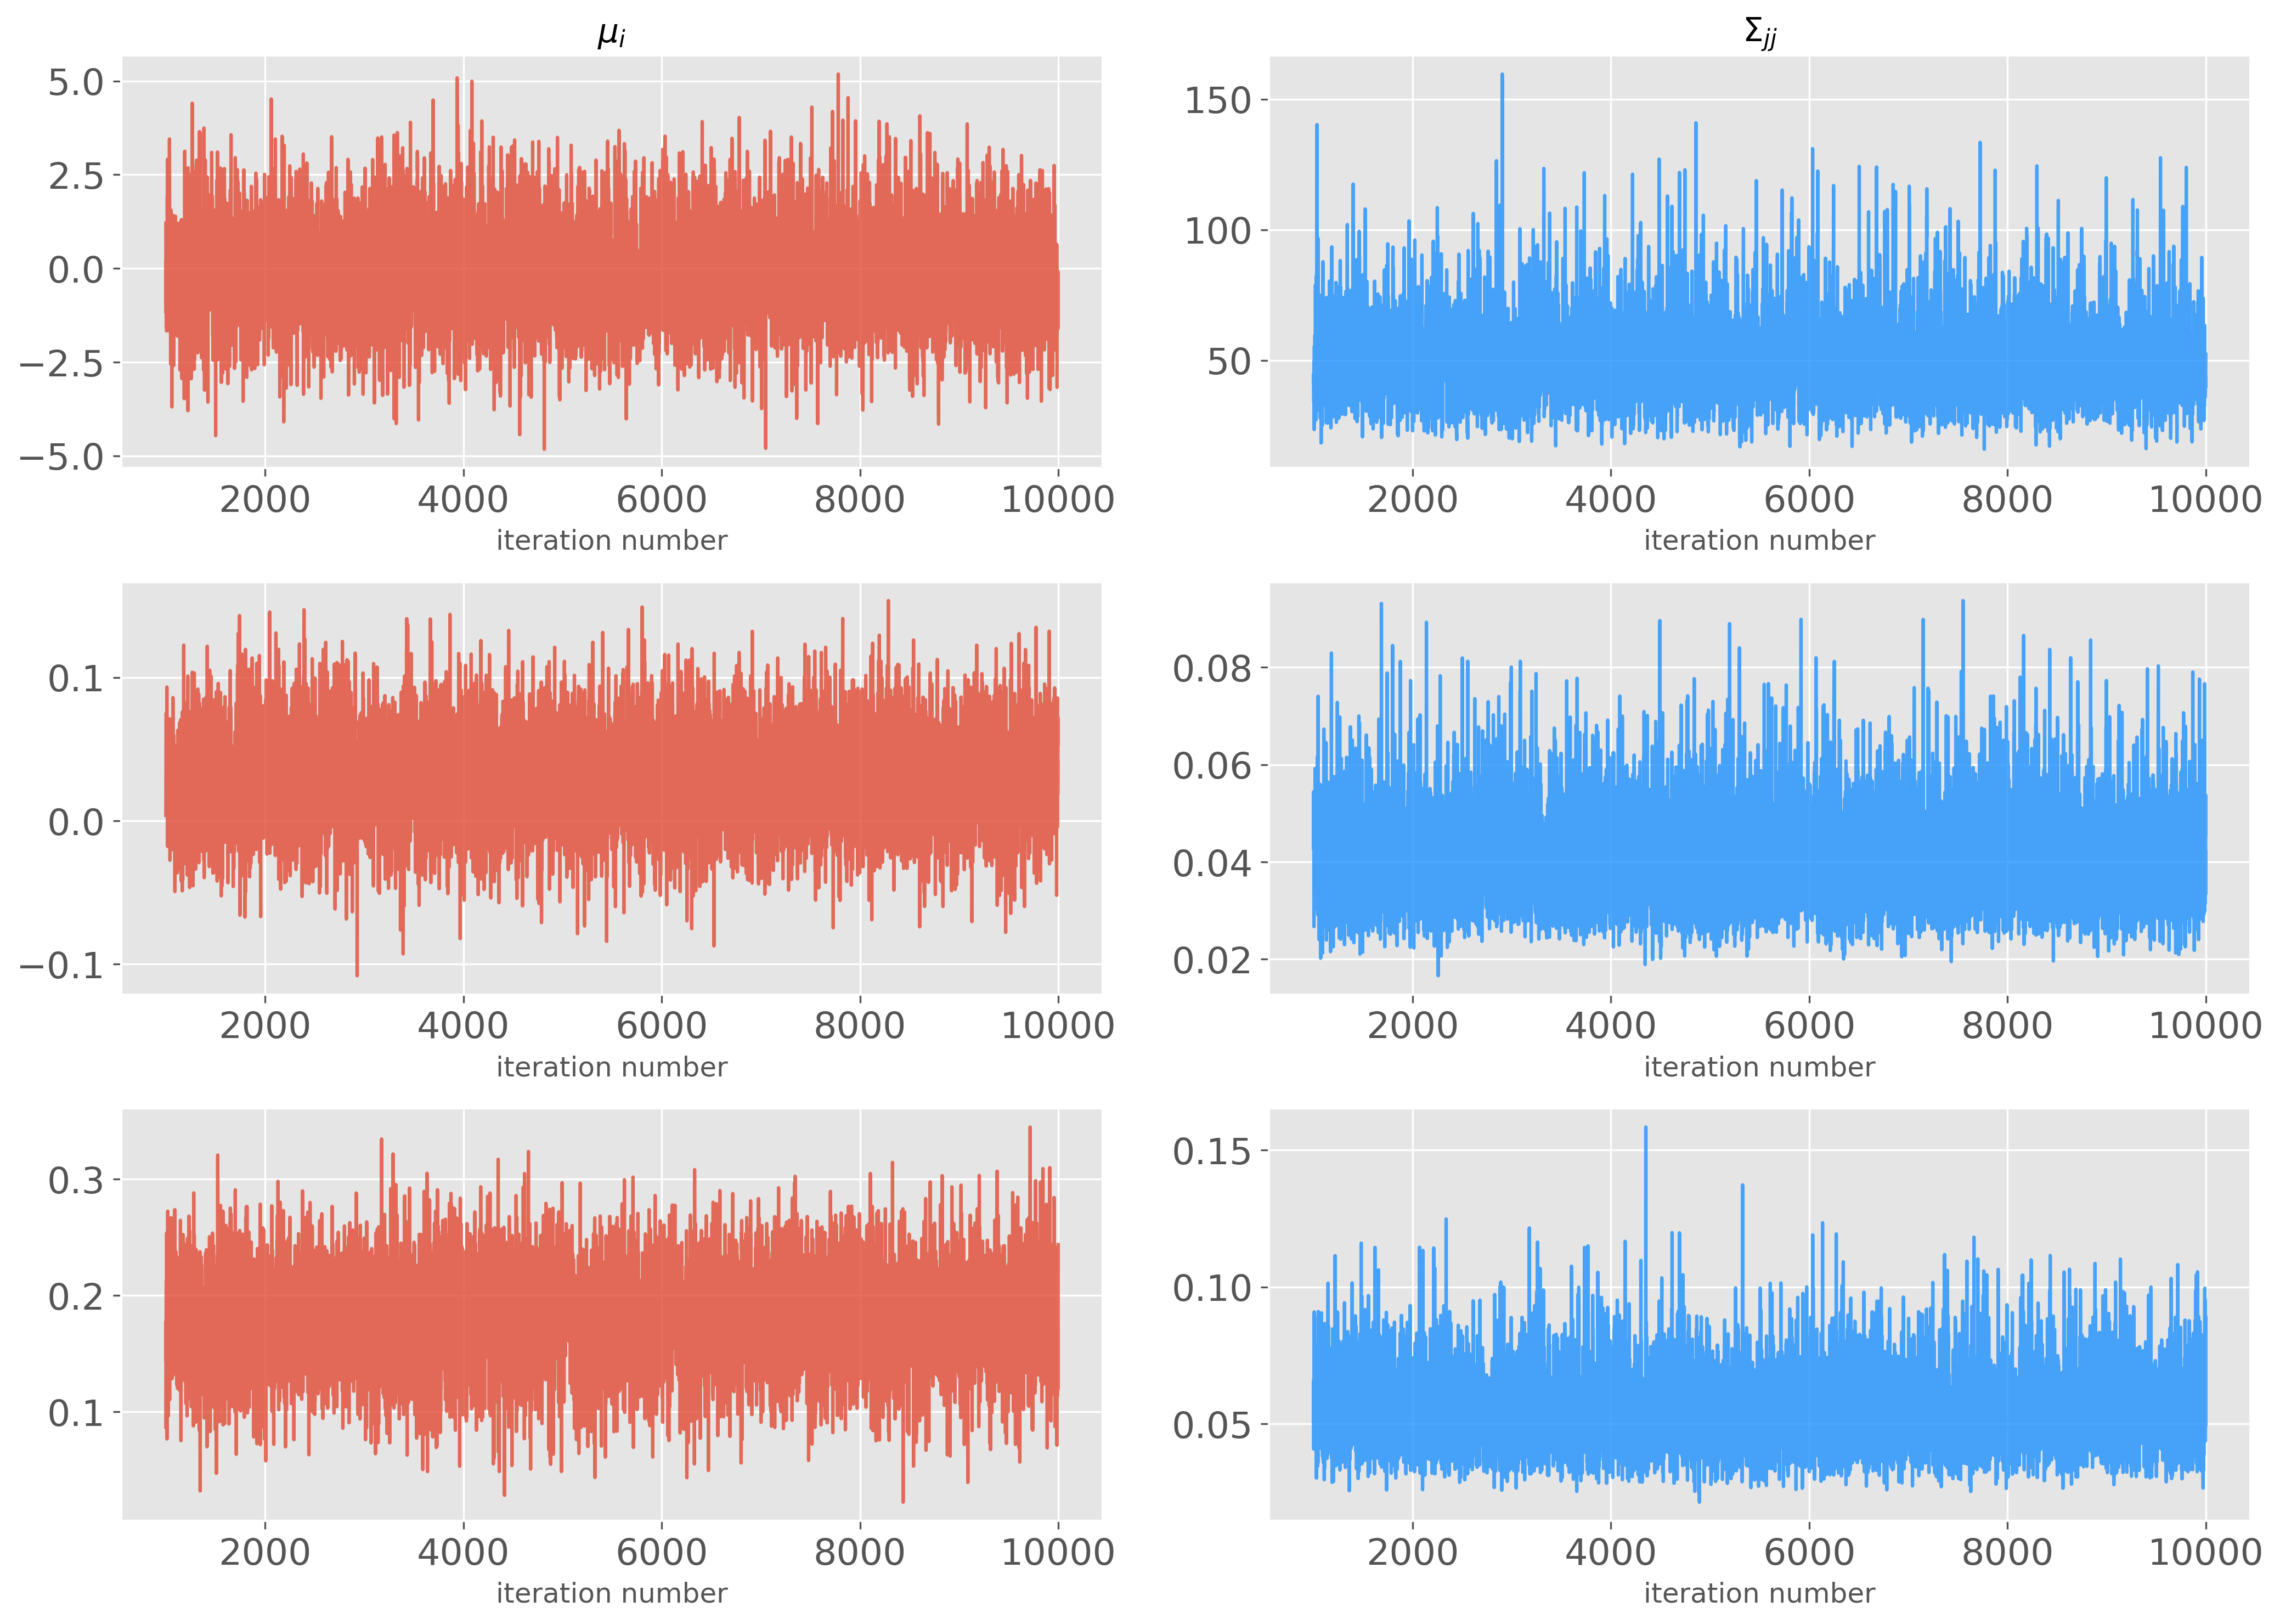
\includegraphics[width=1\textwidth]{project/writeup/traces_simple_model.png}
\caption{Traces for $\mu$ and $\mu_{jj}$}
\end{figure}


The Gibbs sampler was also compared to the PyMC results. The posteriors looked very similar, except the posteriors for $\mu_2$ and $\Sigma_{22}$, as shown in Figure \ref{pymc1}. However, the posteriors for $\beta_2$ looked fairly similar as shown in Figure \ref{pymc2}. The differences may be due to the fact that the priors on $\sigma^2_i$ were different.

\begin{figure}[!htb]\label{pymc1}
\centering
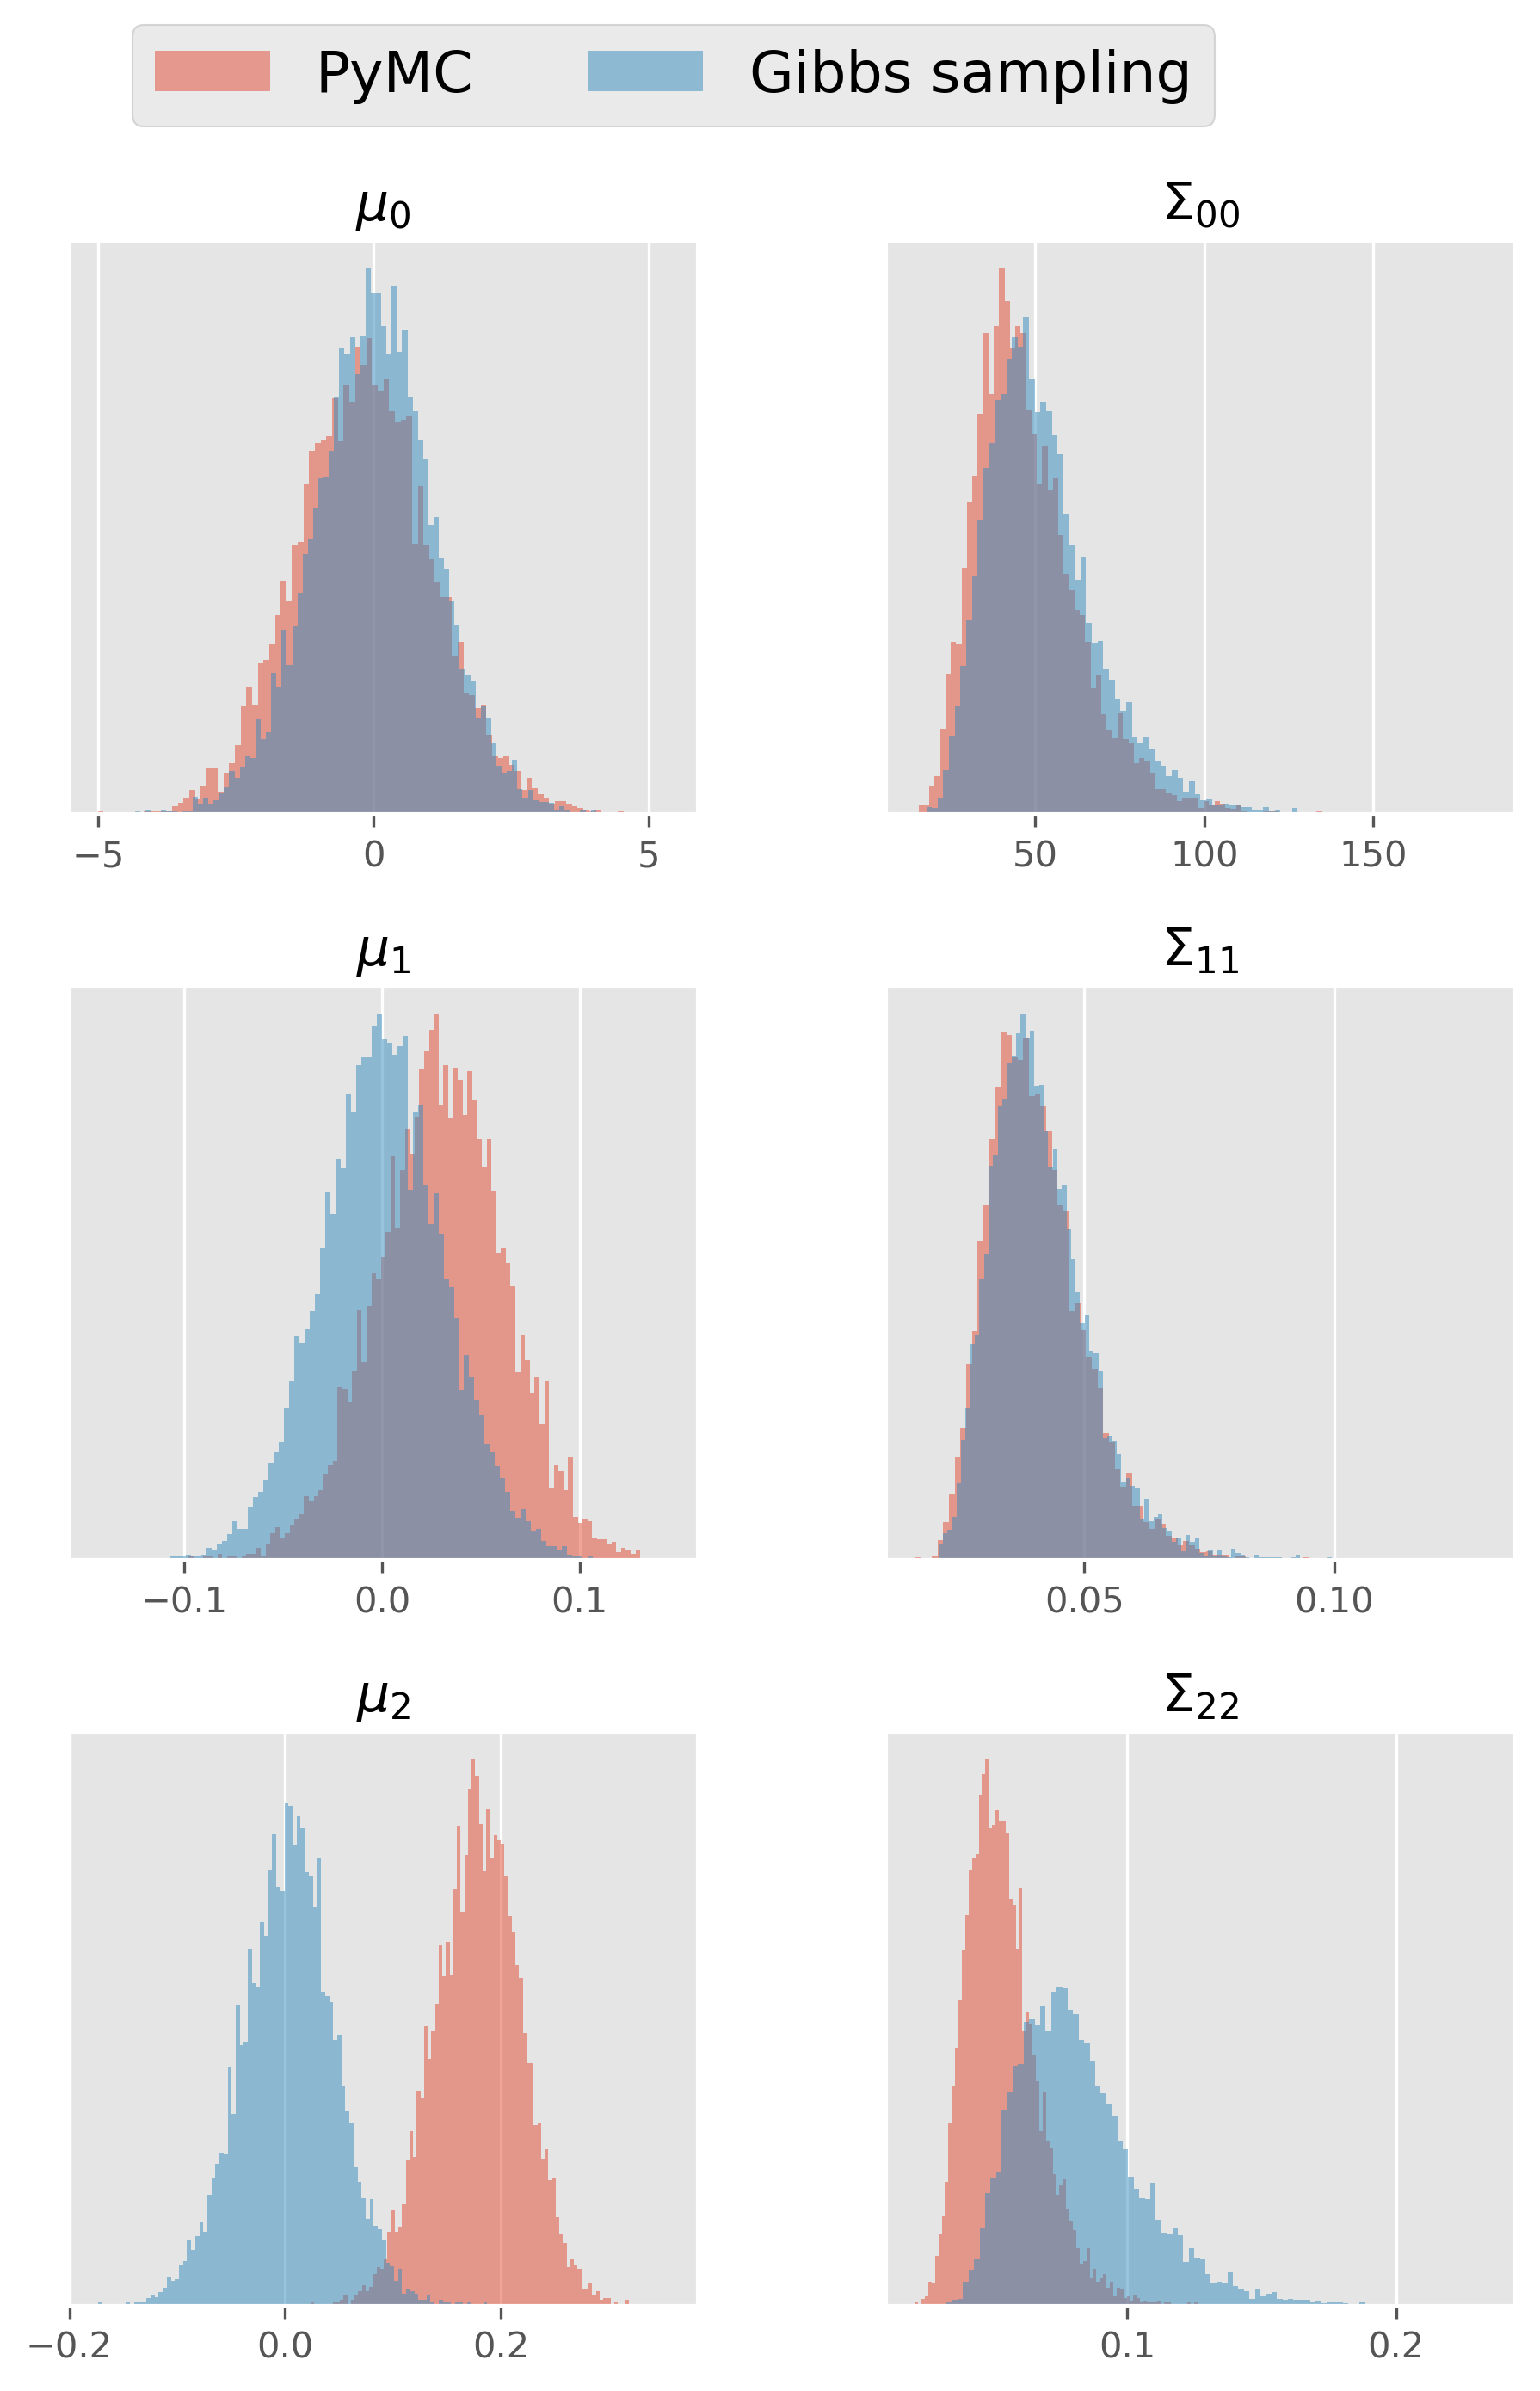
\includegraphics[width=.4\textwidth]{project/writeup/compare_gibbs_pymc1.png}
\caption{Posteriors for $\mu$ and $\Sigma$}
\end{figure}


\begin{figure}[!htb]\label{pymc2}
\centering
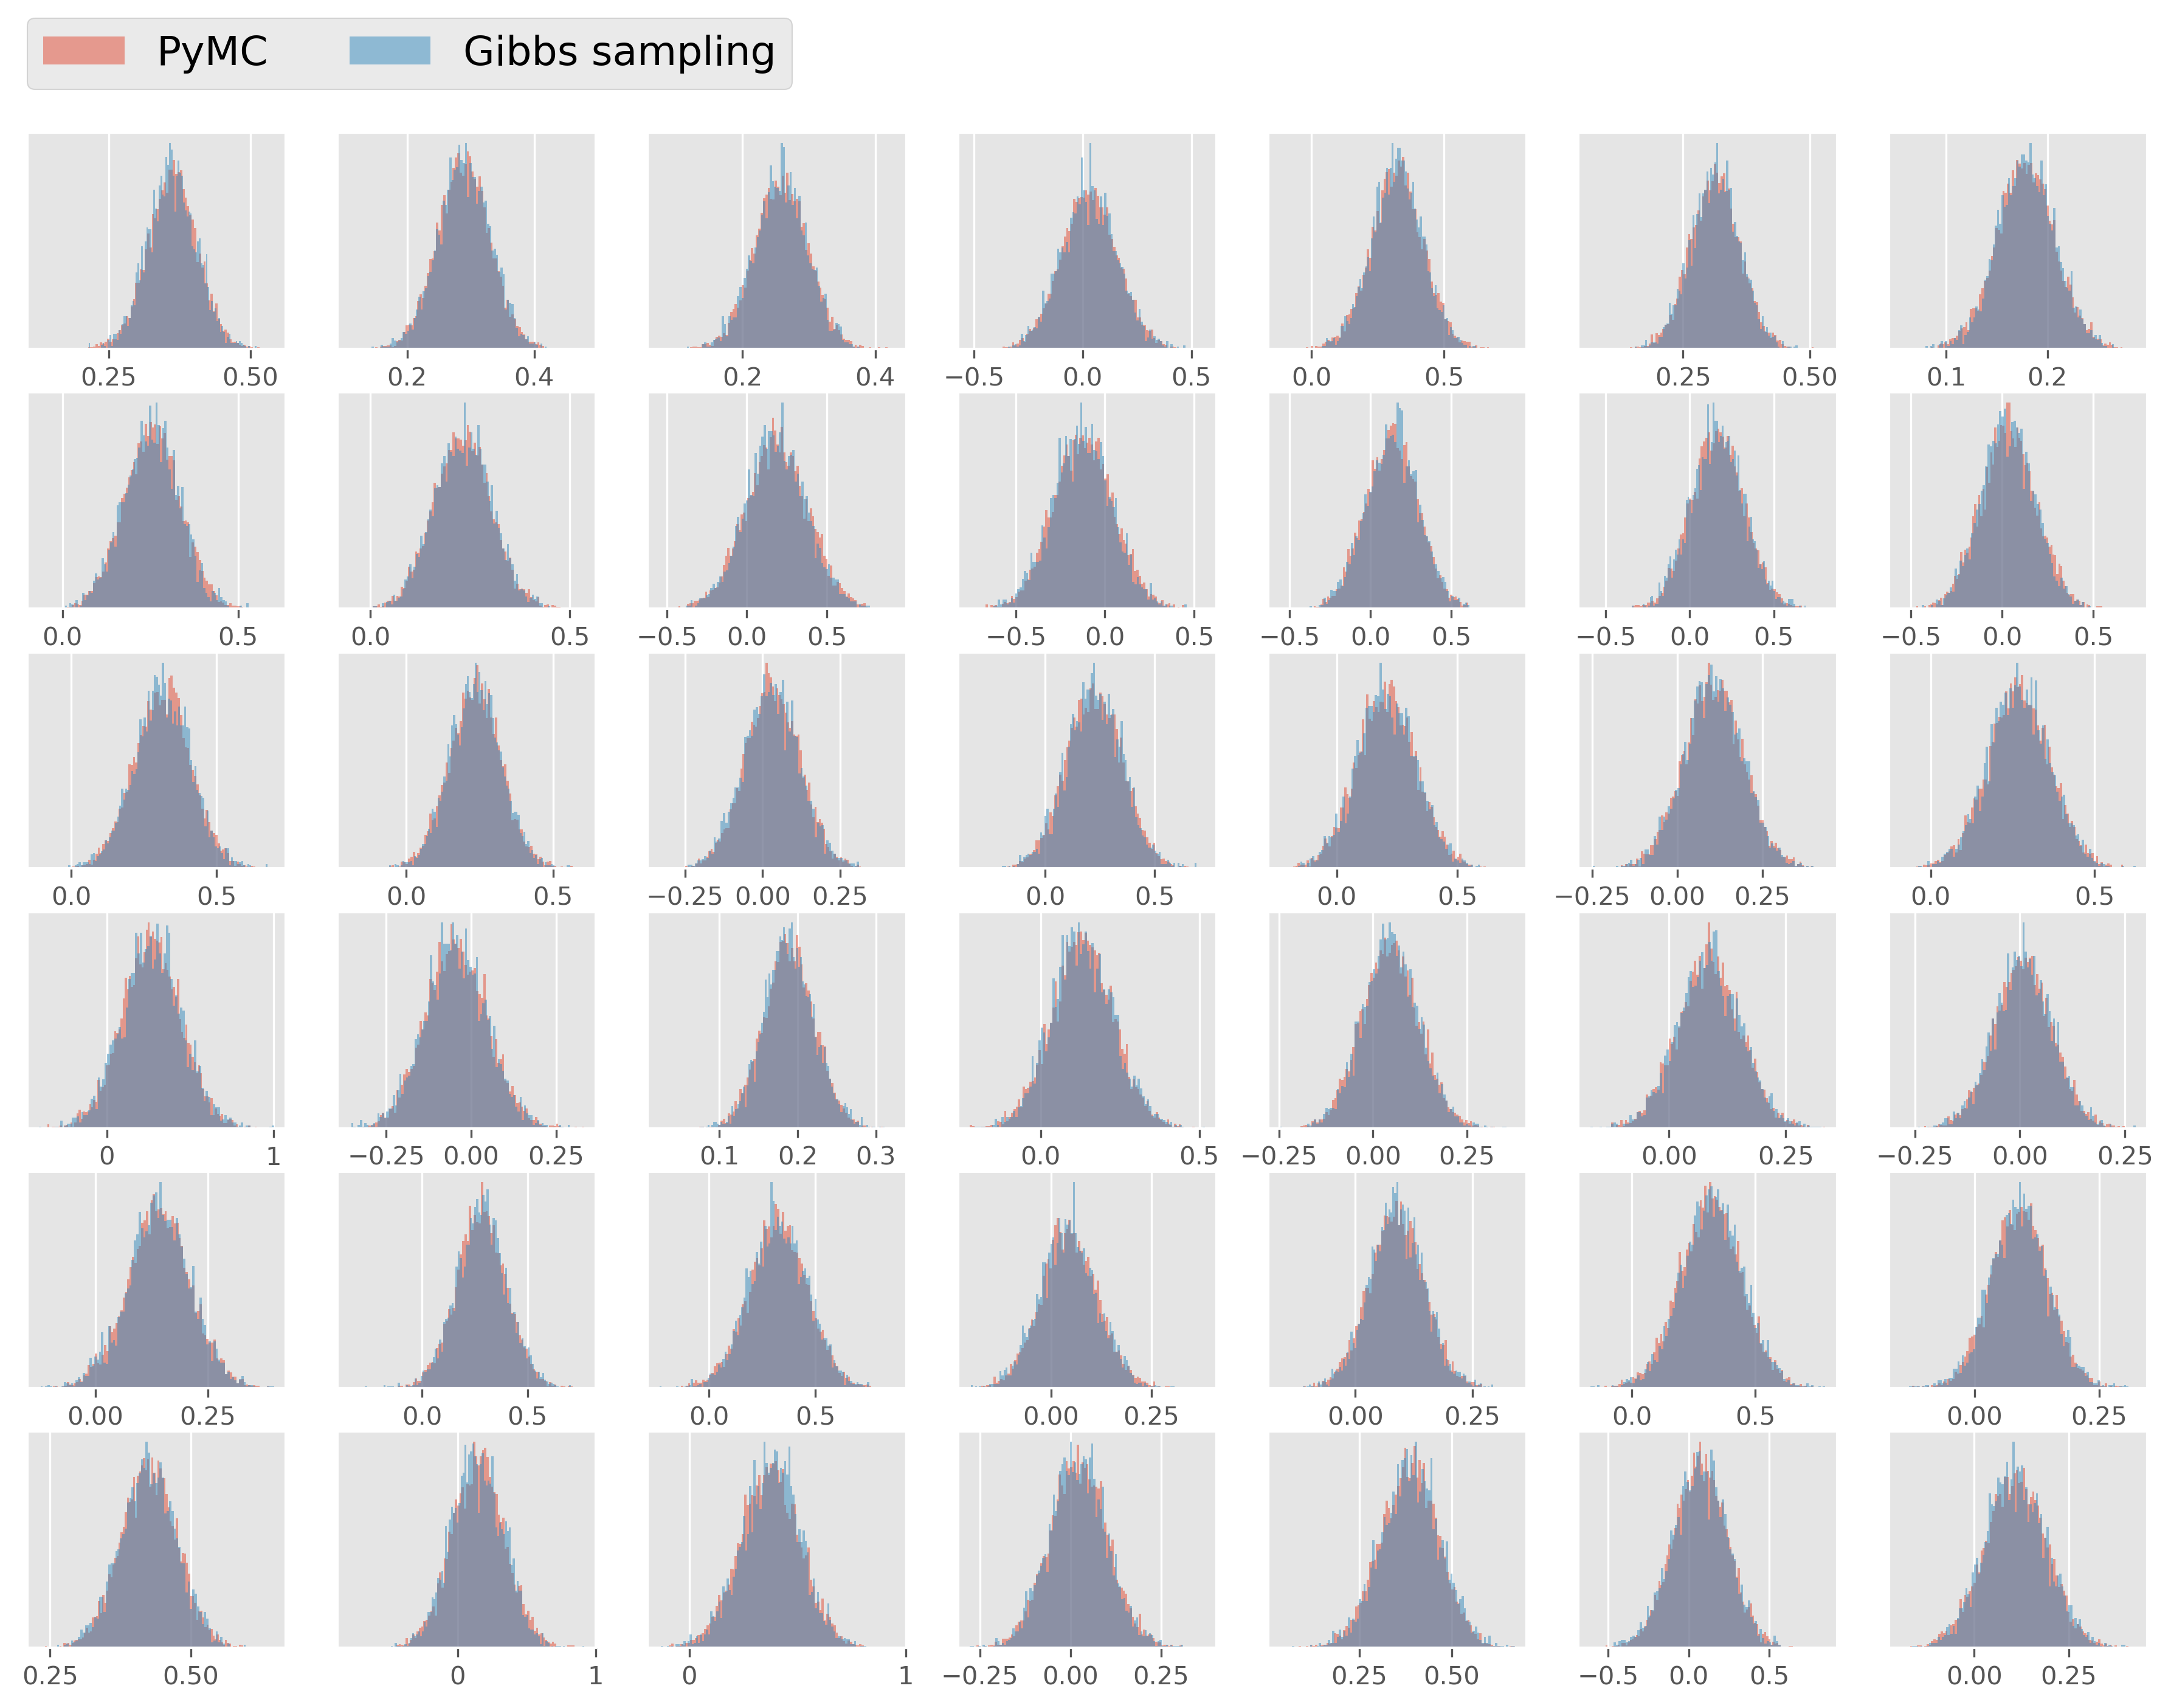
\includegraphics[width=1\textwidth]{project/writeup/compare_gibbs_pymc2.png}
\caption{Posteriors for $\beta_2$}
\end{figure}



\subsubsection{Gaussian Process Model}
The Gaussian Process Hierarchical model was run four separate times to verify that the traces converged to the same posterior distributions. However, major issues were encountered with the model. Traces, especially for the bandwidths and $\tau^2_i$ were not well mixed, and the traces for the four chains did not converge to the same distribution. Additionally, the acceptance rates for the bandwidths and $\tau^2_i$ were too high for Metropolis-Hastings (>0.9). Attempts were made to fix the issues encountered: several variances in the proposal distributions were tested and the model was run for as long as possible given time constraints (150,000 iterations). However, the issues remained. The issues discussed are illustrated in the plots below. Selected traces for one department only is shown due to space constraints, but the issue occurred in almost all 42 departments.\\

Figure \ref{b} shows the traces for the bandwidth for department number 13. The traces are not well-mixed and the four chains did not seem to converge to the same posterior. Unsurprisingly, the Gelman-Rubin convergence diagnostic is not acceptable (1.25, which is above the commonly used cut-off of 1.1). Note that when calculating the diagnostic, the right 5,000 iterations were omitted. The chains for  $\tau^2$ looked more mixed but also did not converge; their Gelman-Rubin diagnostic was 1.35. The traces for $\beta_0$ were better, but not those for $\beta_1$ and $\beta_2$. The traces for $\sigma_i^2$ looked well-mixed but only after about 60,000 iterations. The traces for the first element of $f$ were also well mixed and had an acceptable Gelman-Rubin diagnostic.





\begin{figure}[!htb]\label{b}
\centering
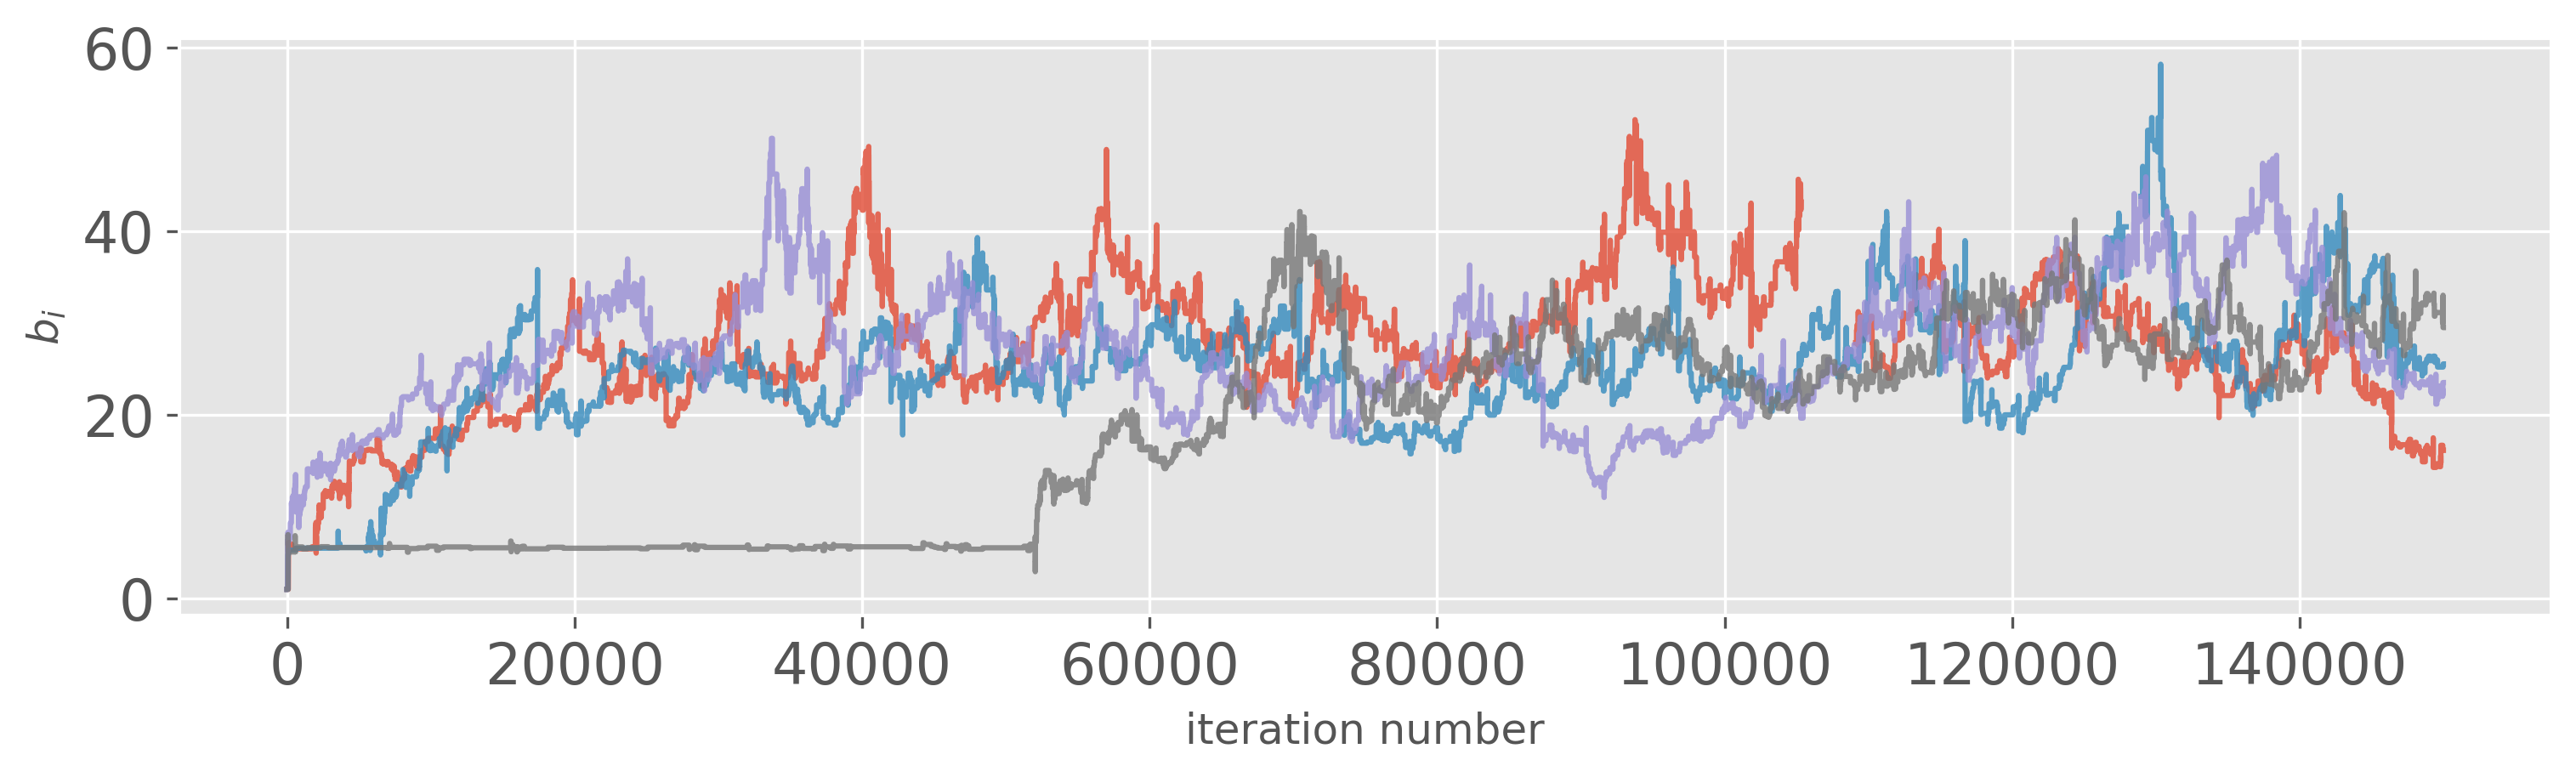
\includegraphics[width=1\textwidth]{project/writeup/bandwidth.png}
\caption{Traces for the bandwidth for department number 13}\end{figure}



\begin{figure}[!htb]\label{tau}
\centering
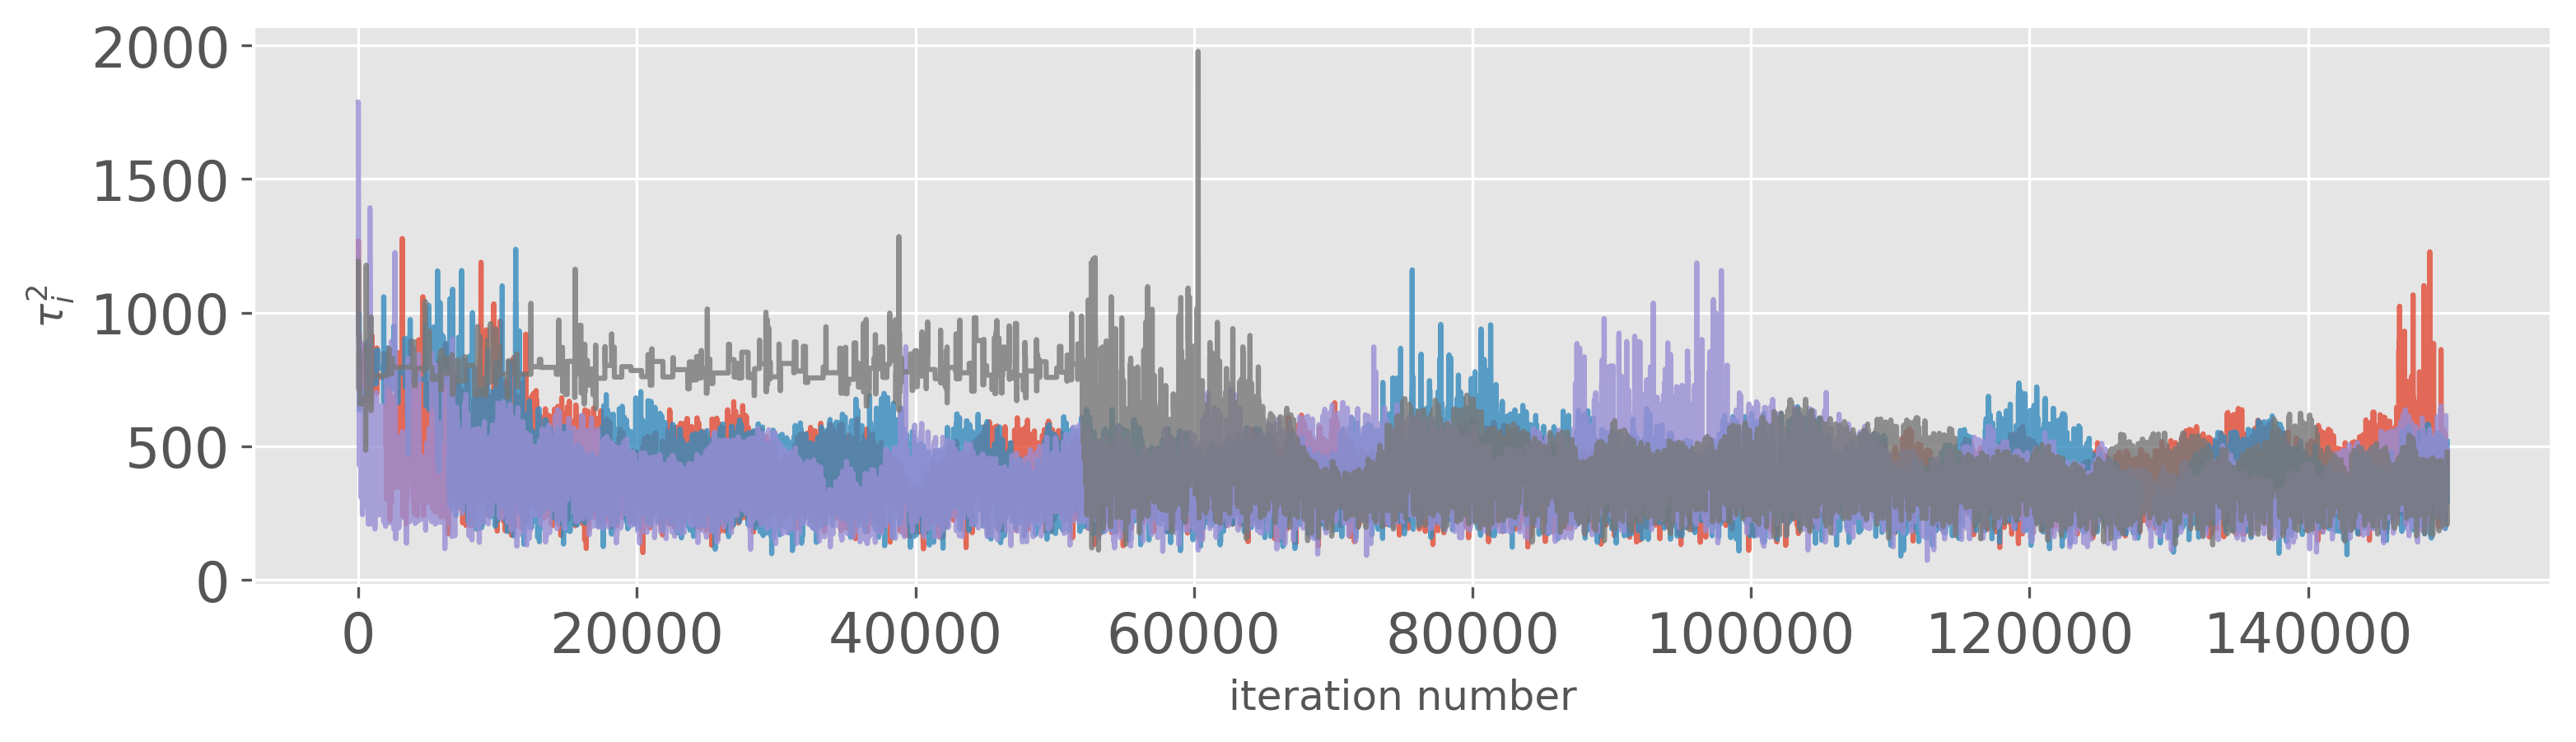
\includegraphics[width=1\textwidth]{project/writeup/tau.png}
\caption{Traces for $\tau^2$ for department number 13}\end{figure}


\begin{figure}[!htb]\label{beta}
\centering
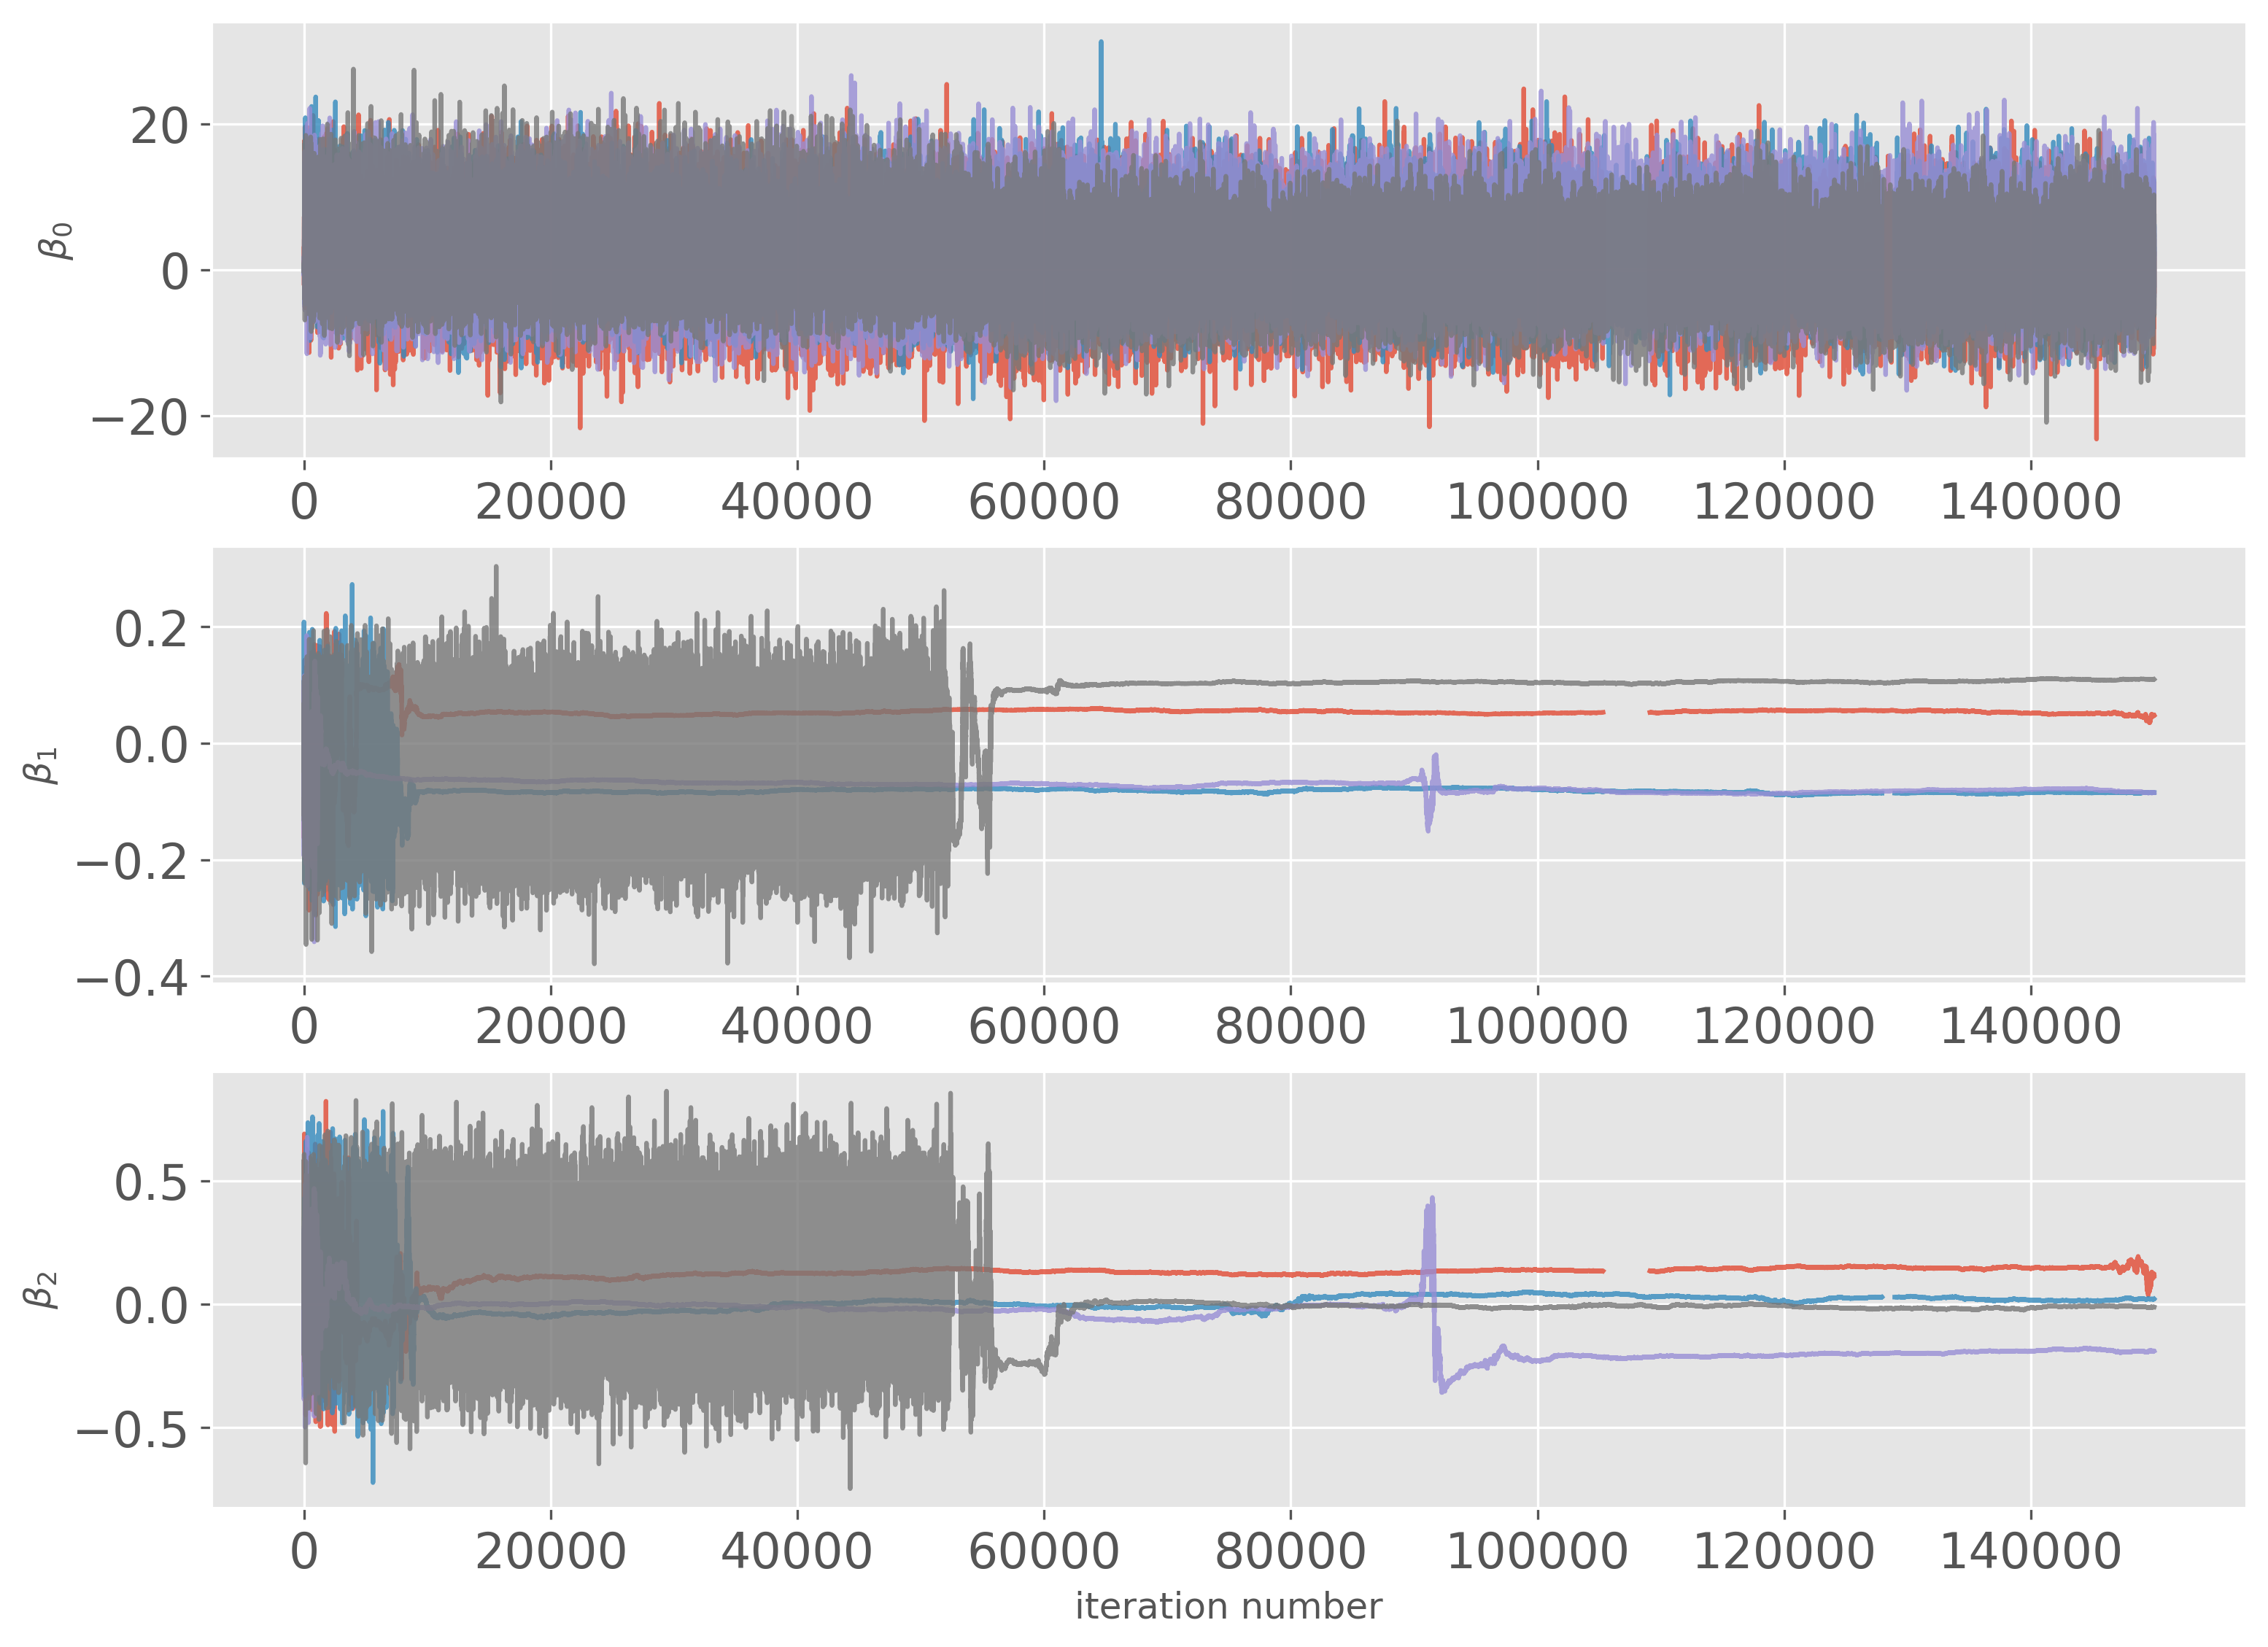
\includegraphics[width=1\textwidth]{project/writeup/betas_traces.png}
\caption{Traces for $\beta$ for department number 13}\end{figure}


\begin{figure}[!htb]\label{sigma}
\centering
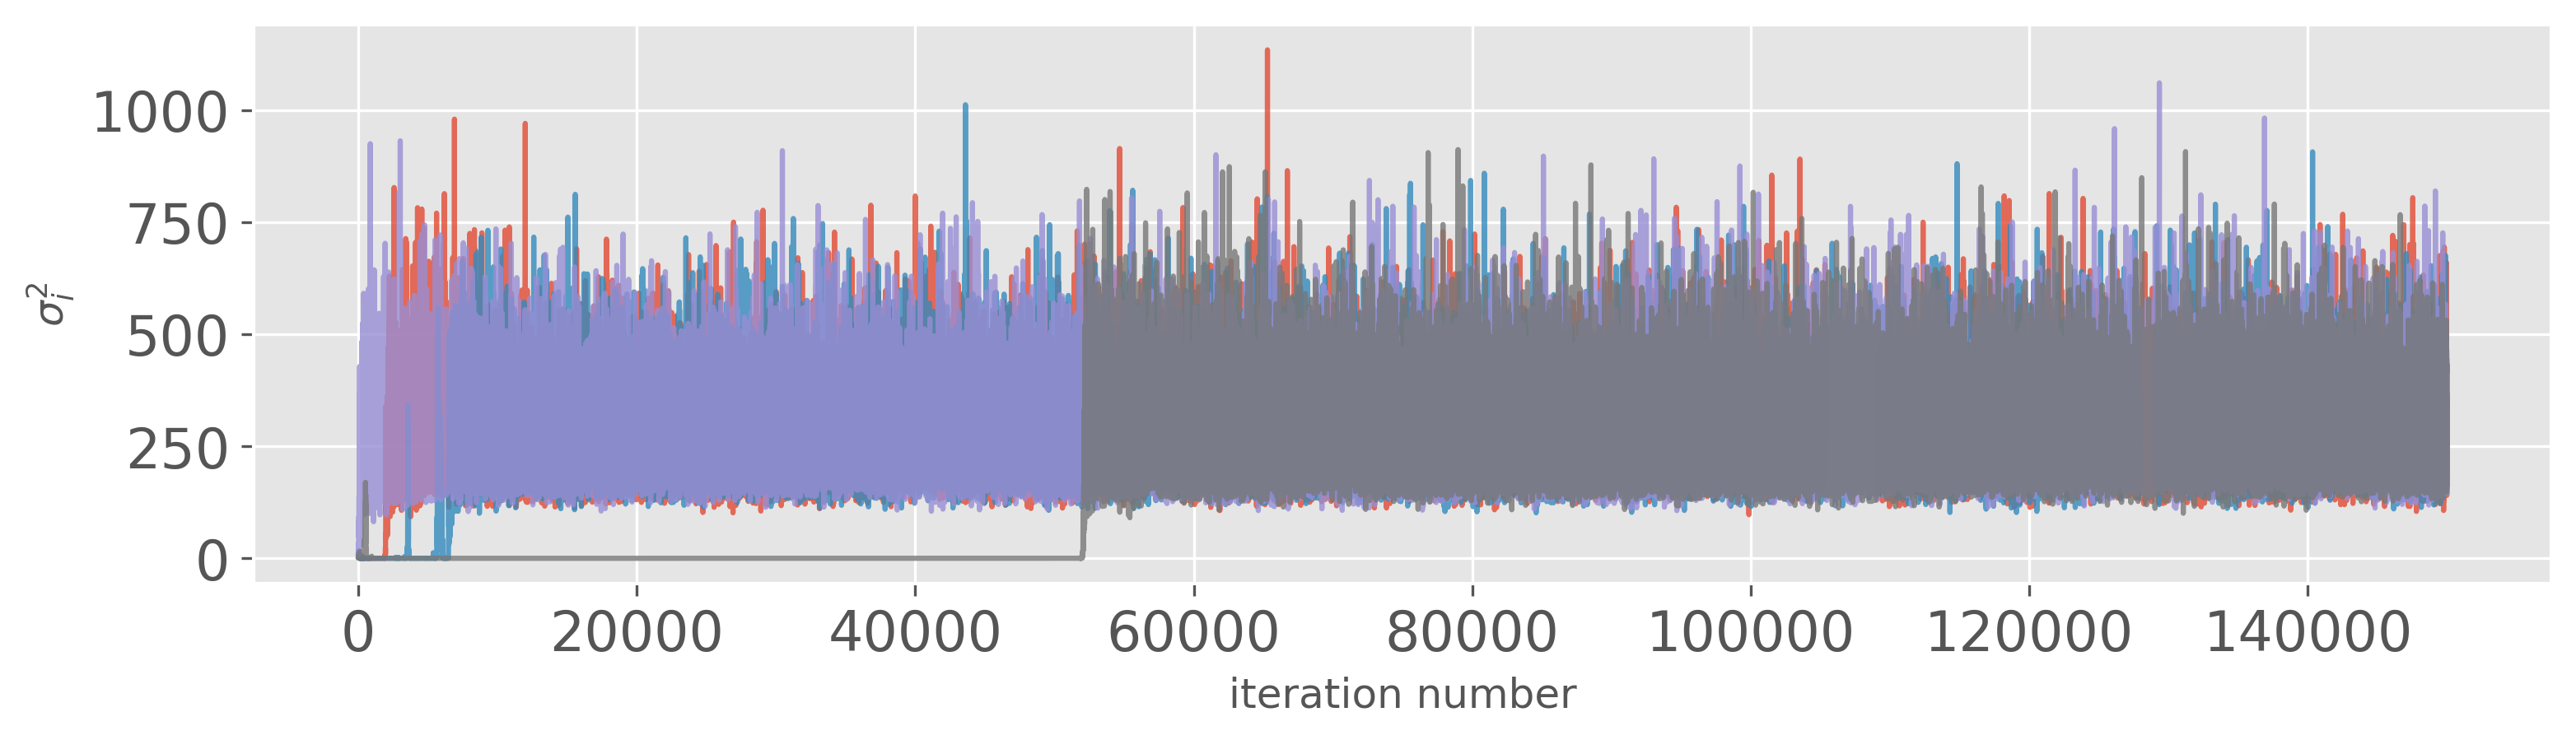
\includegraphics[width=1\textwidth]{project/writeup/sigma.png}
\caption{Traces for $\sigma_i^2$ for department number 13}
\end{figure}

\begin{figure}[!htb]\label{f}
\centering
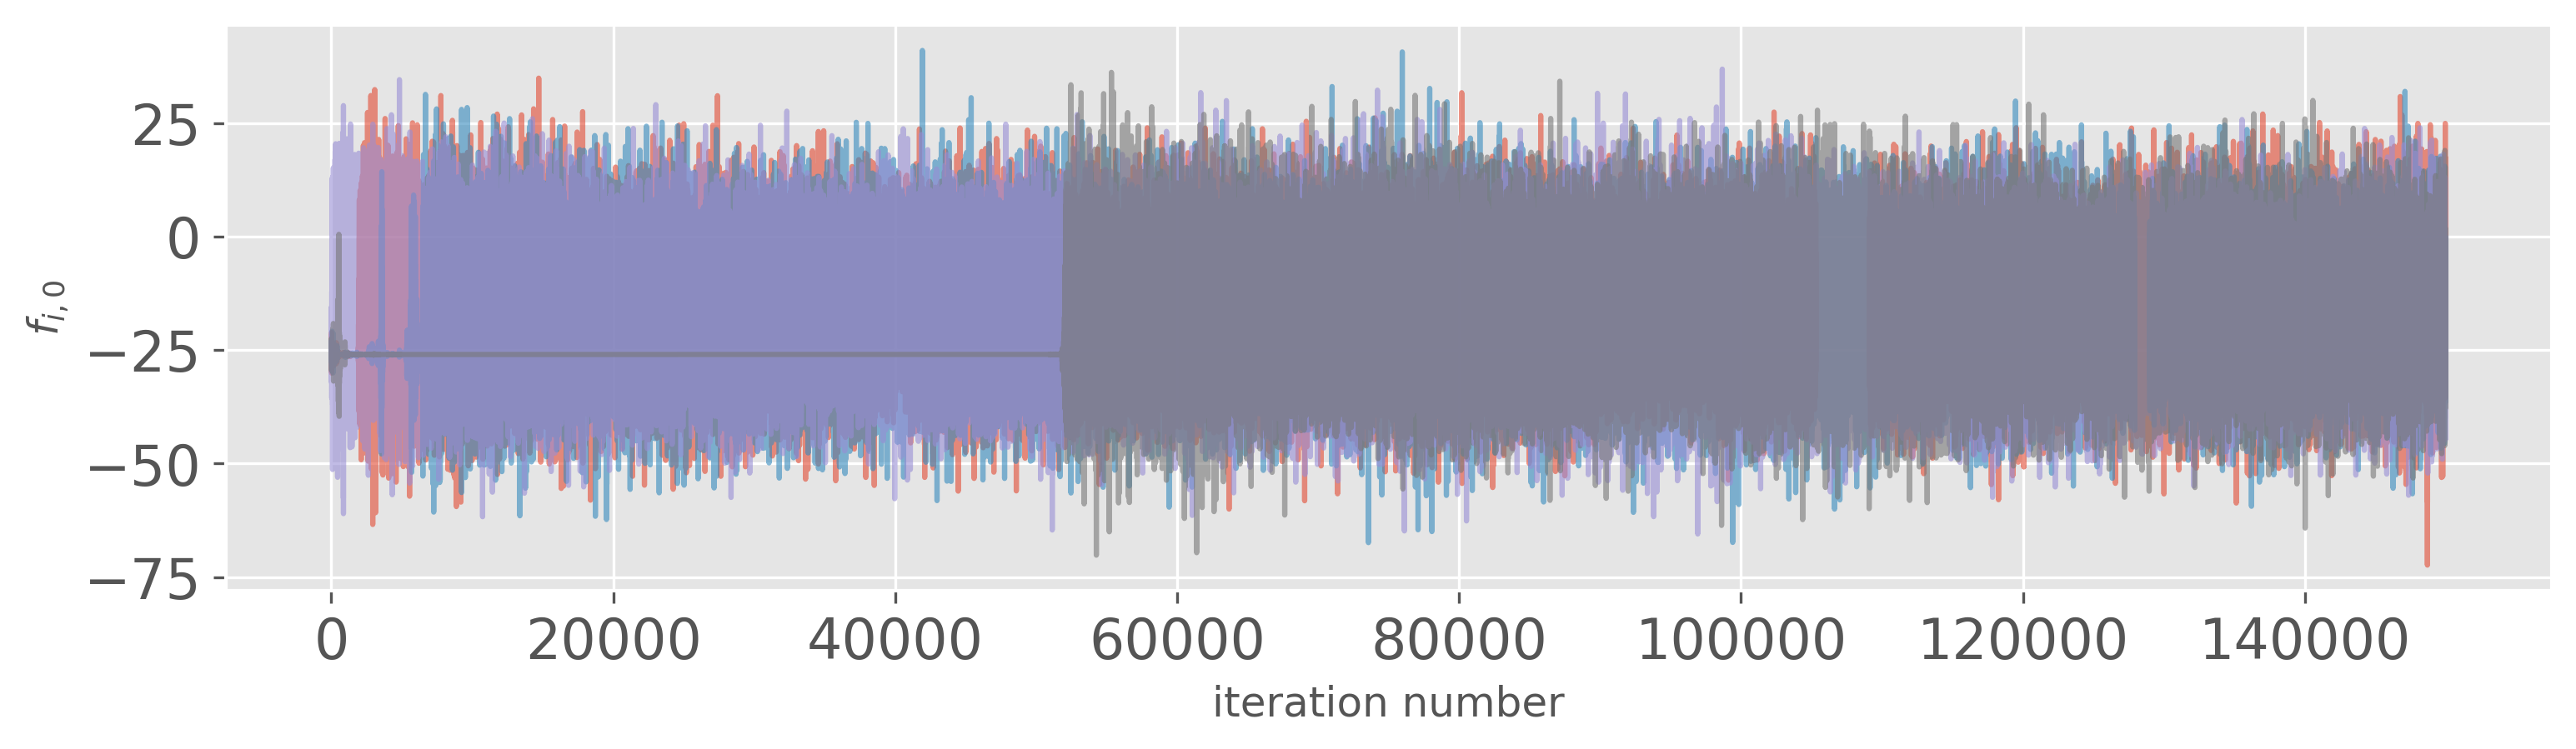
\includegraphics[width=1\textwidth]{project/writeup/f.png}
\caption{Traces for the first element of $f$ for department number 13}\end{figure}




\subsection{Interpretation}


\begin{figure}[!htb]\label{corr_mat}
\centering
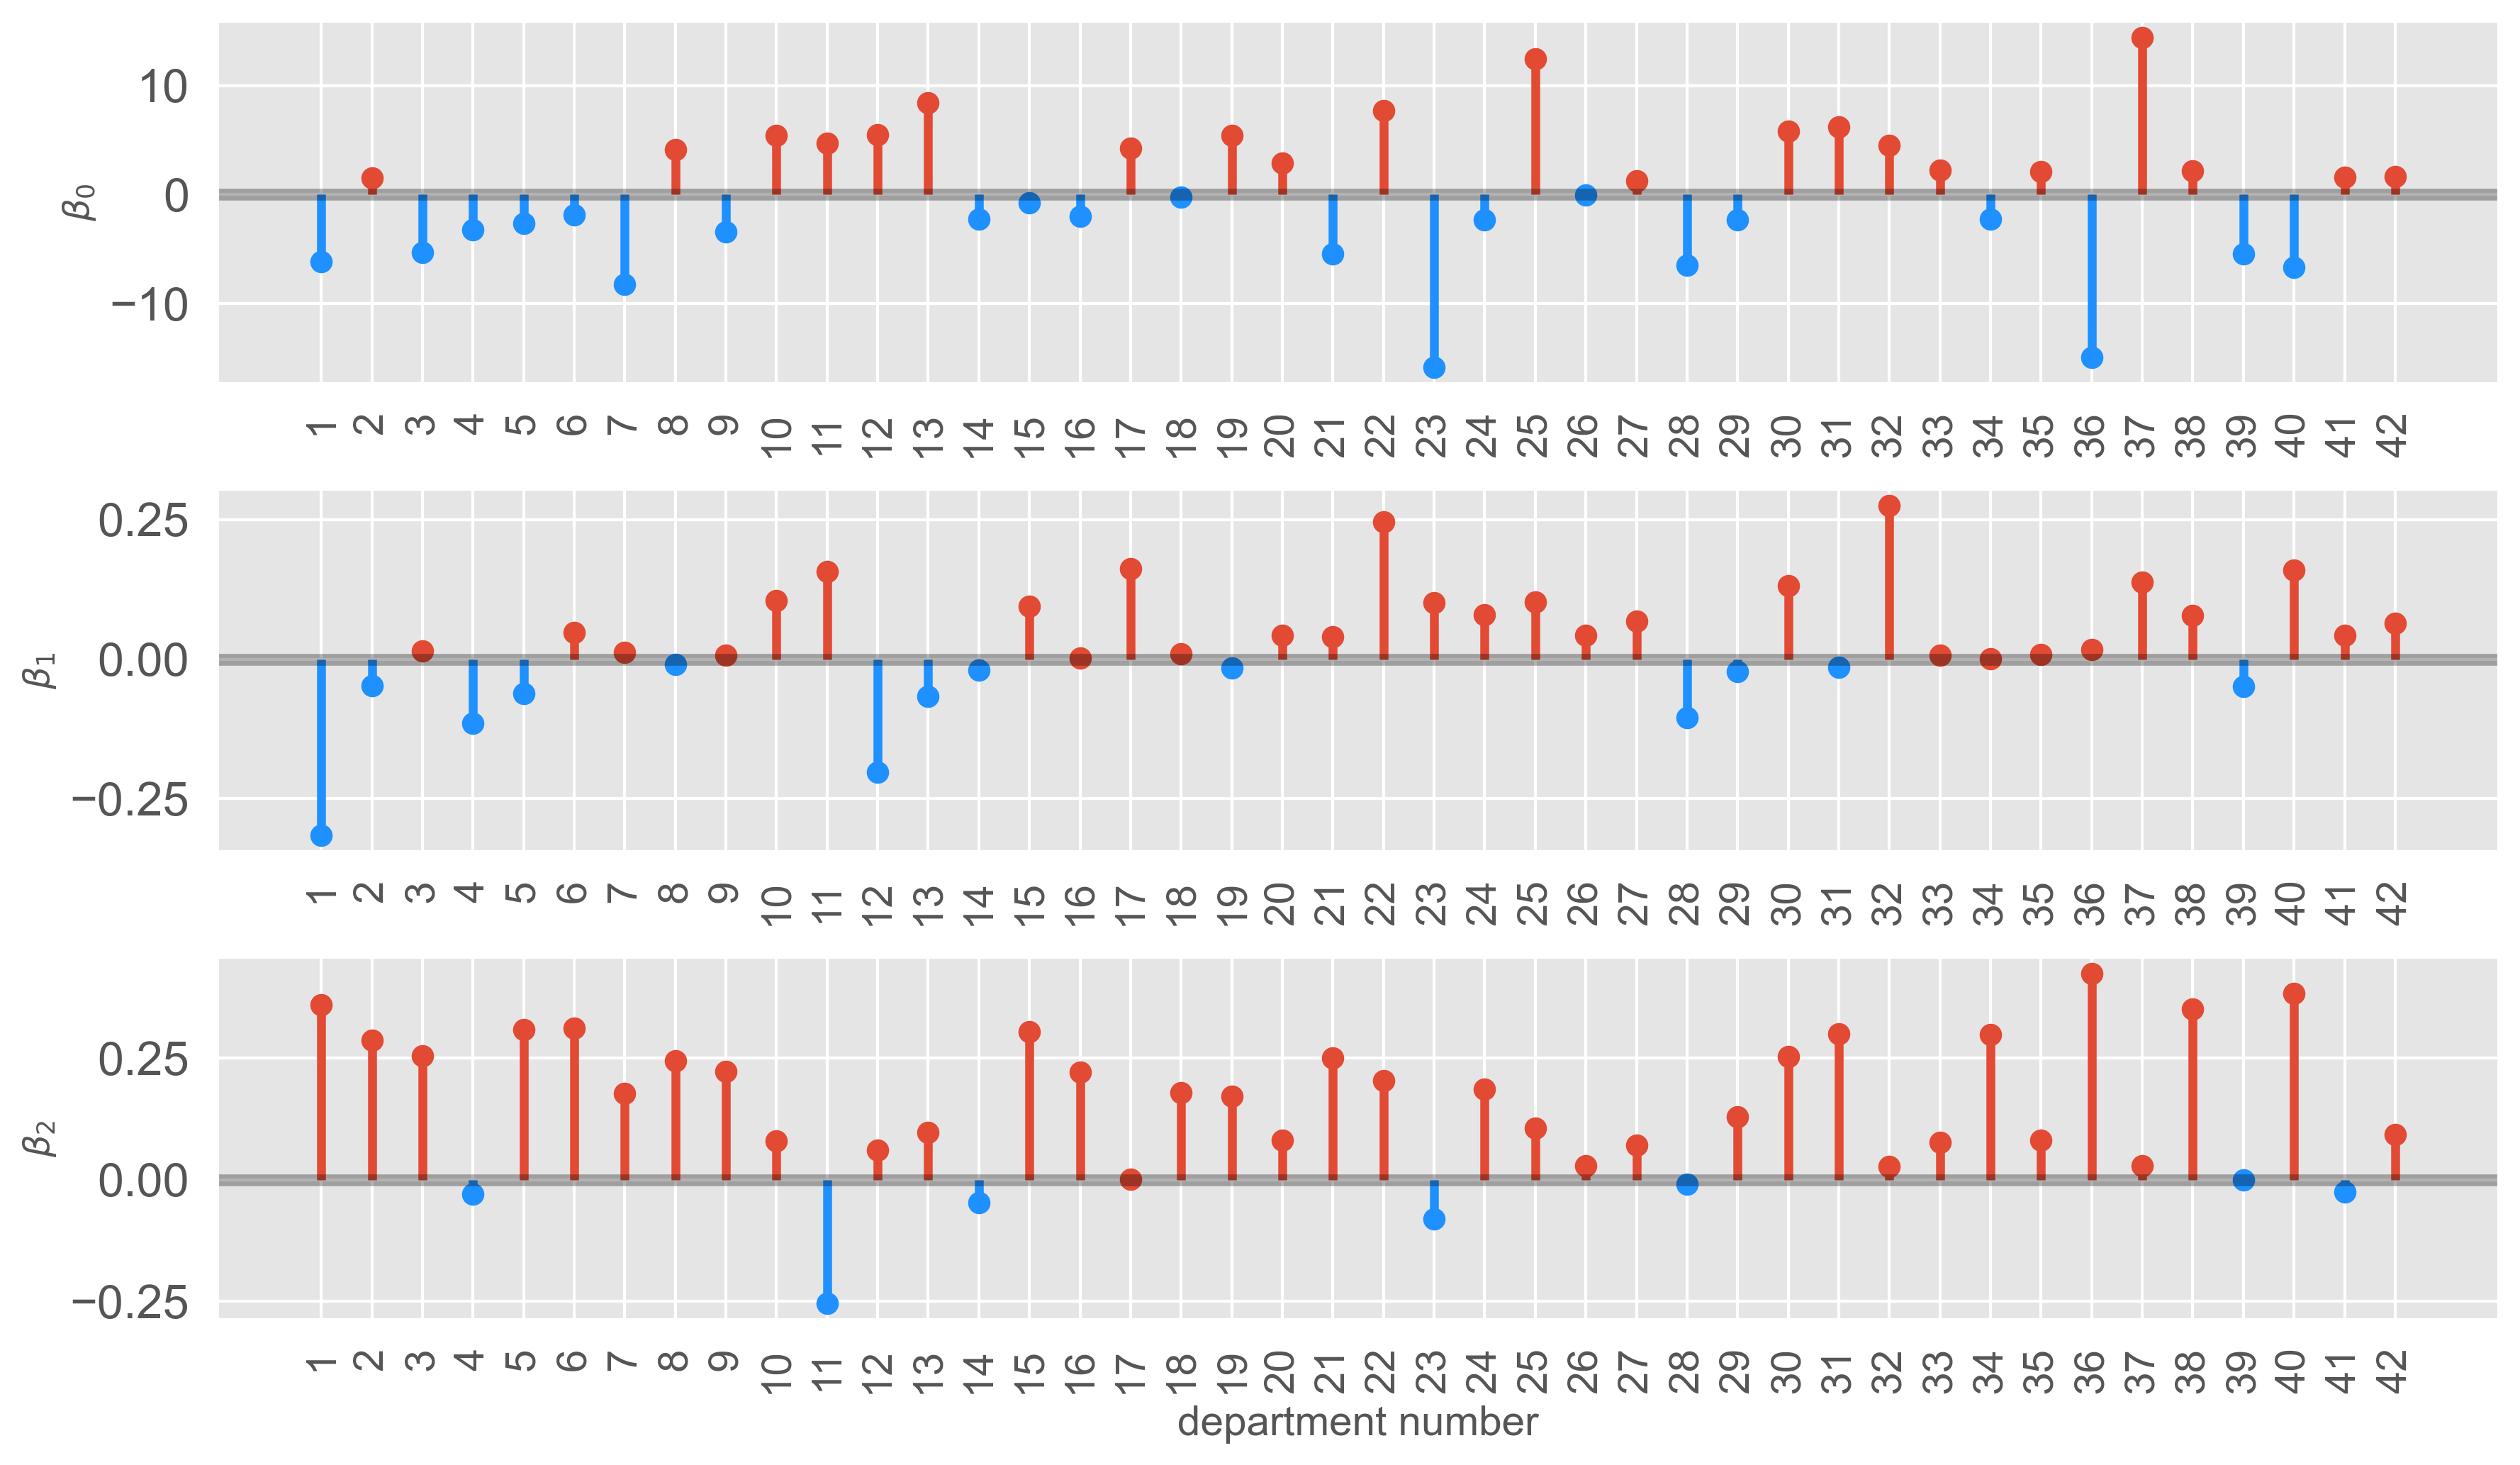
\includegraphics[width=1\textwidth]{project/writeup/mean_betas.png}
\caption{$\beta$ means}\end{figure}


\begin{figure}[!htb]\label{corr_mat}
\centering
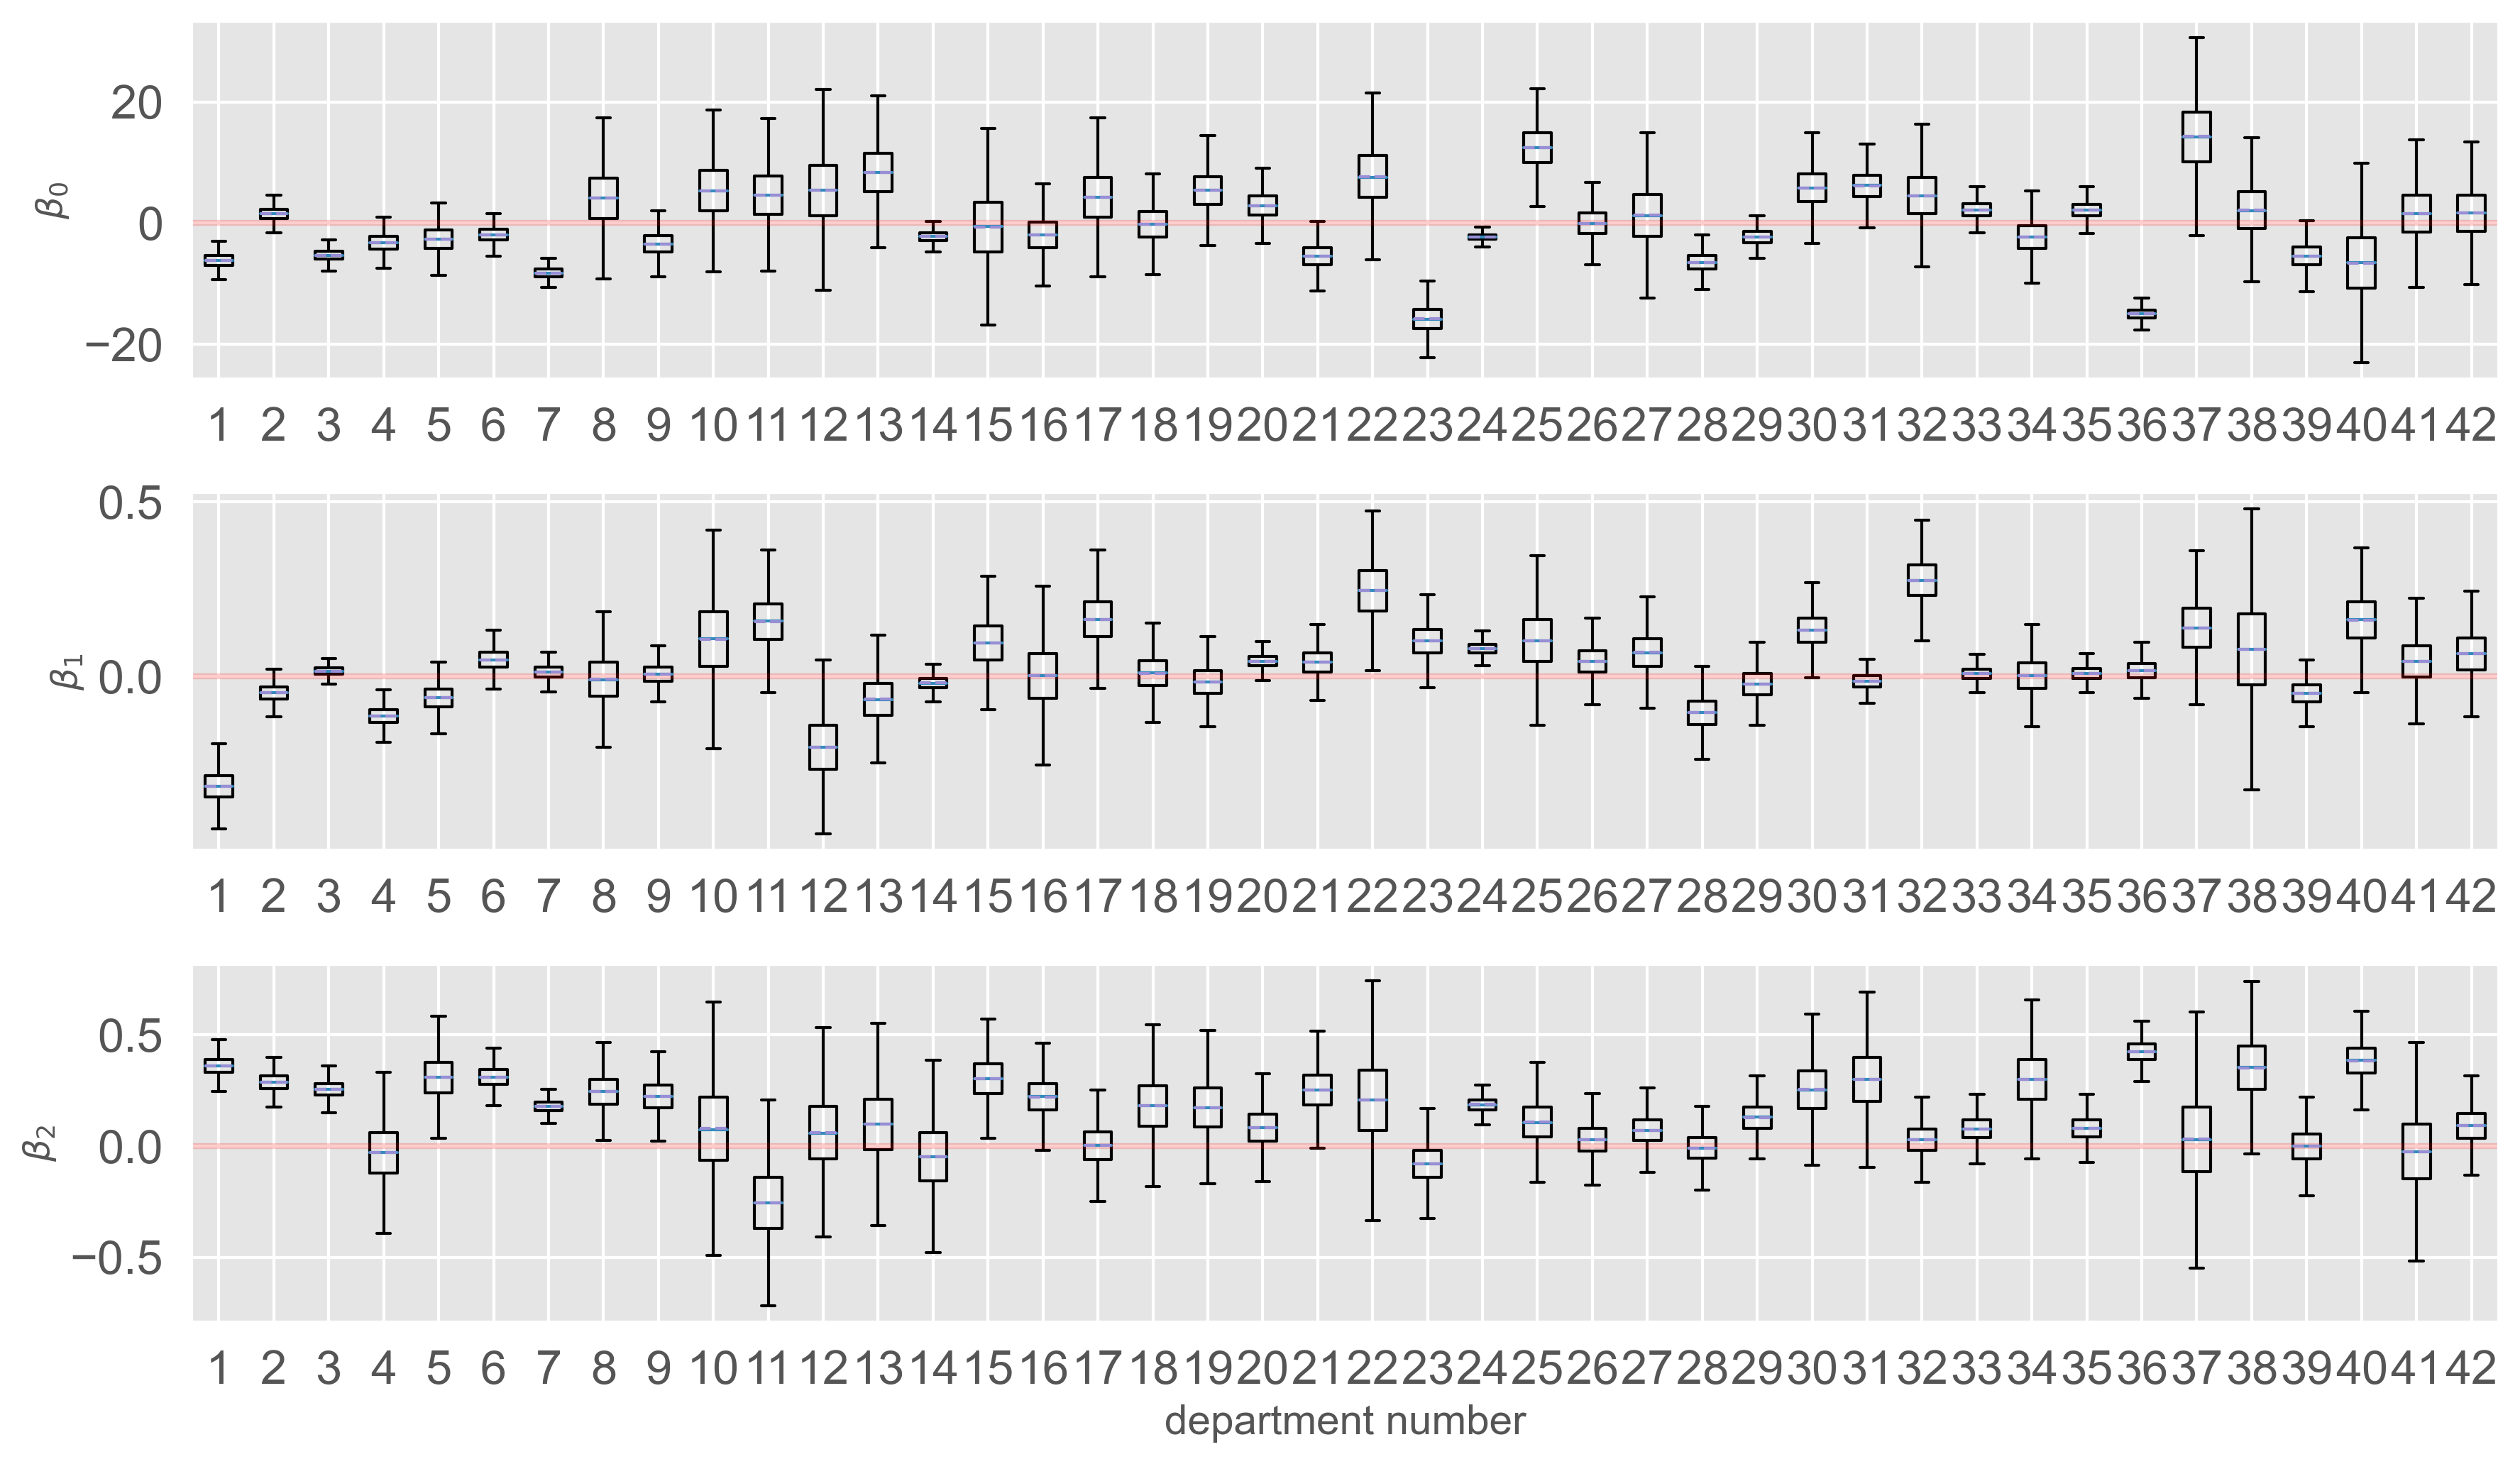
\includegraphics[width=1\textwidth]{project/writeup/box_plots.png}
\caption{$\beta$ boxplots}
\end{figure}


\bibliography{refs} 
\bibliographystyle{ieeetr}

\end{document}